\documentclass[12pt,a4paper]{article}
\usepackage[left=28mm,top=30mm,right=28mm,bottom=27mm]{geometry}
\usepackage{graphicx} % Required for inserting images
\usepackage{amsfonts}
\usepackage{amsmath}
\usepackage{pgfplots}
\usepackage{flafter}
\usepackage{listings}
\usepackage{xcolor}
\definecolor{codegreen}{rgb}{0,0.6,0}
\definecolor{codegray}{rgb}{0.5,0.5,0.5}
\definecolor{codepurple}{rgb}{0.58,0,0.82}
\definecolor{backcolour}{rgb}{0.94,0.94,0.95}
\lstdefinestyle{mystyle}{
    backgroundcolor=\color{backcolour},   
    commentstyle=\color{codegreen},
    keywordstyle=\color{magenta},
    numberstyle=\tiny\color{codegray},
    stringstyle=\color{codepurple},
    basicstyle=\ttfamily\footnotesize,
    breakatwhitespace=false,         
    breaklines=true,                 
    captionpos=b,                    
    keepspaces=true,                 
    numbers=left,                    
    numbersep=5pt,                  
    showspaces=false,                
    showstringspaces=false,
    showtabs=false,                  
    tabsize=2
}
\lstset{style=mystyle}
\usepackage{breakcites}
\usepackage[font=footnotesize]{caption}
\usepackage[T1]{fontenc}
\usepackage{XCharter}
\usepackage{setspace}
\usepackage[pdftex]{hyperref}
\hypersetup{
    colorlinks=true,
    linkcolor=red,
    citecolor=blue,
    urlcolor=cyan
}


\title{Replication of Token Merging for fast Stable Diffusion}
\author{Henri Balster}
\date{}
\begin{document}
\pagenumbering{gobble}
\begin{titlepage}
    \centering
    
\includegraphics[width=10cm]{static/Logo_HHU_+Name_horizontal_4c_+Safezone}\\

    \vspace*{2cm}

    \huge
    \textbf{Replication of Token Merging for fast Stable Diffusion}
    
    \large
    \vspace{1cm}
    Thesis Subtitle
            
    \vspace{1.5cm}

    \textbf{Henri Balster}

    \vfill
            
    A thesis presented for the bachelor's\\
    degree of Computer Science
            
    \vspace{0.8cm}
            
    Department Name\\
    Dr. Konrad Völkel\\
    Heinrich-Heine-Universität Düsseldorf\\
    Date
            
\end{titlepage}
\newpage
\tableofcontents
\onehalfspacing
\newpage
\pagenumbering{arabic}

\begin{table}[!htb]
\centering
\begin{tabular}{c c c}
    
\includegraphics[width=0.3\linewidth]{static/sample_imgs/main/wookie_0.png} & 
\includegraphics[width=0.3\linewidth]{static/sample_imgs/main/wookie_20.png} &
    
\includegraphics[width=0.3\linewidth]{static/sample_imgs/main/wookie_50.png}\\
    \(r=0\%\) & \(20\%\) & \(50\%\) \\
\end{tabular}
\caption{$768 \times 768$ images created with the default configuration of ToMe}
\end{table}

\section*{Abstract}
%General Background:
Image generation models, such as Stable Diffusion, are popular tools for creating any desired image from a line of text. 
%Specific Background:
The inclusion of new transformer-based technologies into these models has improved the quality of their images, though their operating time can be very slow.
%Knowledge Gap:
\cite{bolya2023tomesd} have introduced Token Merging (ToMe) for Stable Diffusion to improve computational time by reducing the number of tokens evaluated by the model.
%Here we show...:
The goal of this thesis was to replicate their results and investigate whether performance can be improved by using different configurations for ToMe.
%Results:
Our results show that ToMe's default configuration maintains great image quality (most of the time), while accelerating image generation by up to $2.2 \times$, when reducing the number of tokens by up to \(60\%\). Beyond that, we identified different configurations for ToMe that improve the performance compared to the default setup, by using different partitioning methods and expanding the scope of token merging in the transformer. 
%Implications:
This work further solidifies the viability of token merging in diffusion models and incentivises further research into improving the efficiency of transformer based models.
Code and full-scale images are available at \url{https://github.com/HNR1/ba-code}


\section{Introduction}
In this work, our goal is to speed up an off-the-shelf Stable Diffusion model without training using our implementation of token merging (ToMe) \cite{bolya2023tomesd}.
All experiments were conducted on a high performance computing cluster (HPC) provided by the Heinrich-Heine-Universität Düsseldorf.\\
"Even at 60\% of tokens merged, ToMe for SD keeps the image the same (most of the time)"

%\newpage
\section{Background} \label{backgorund}



\subsection{Stable Diffusion}
Stable Diffusion is based on a special type of Diffusion Model called Latent Diffusion Model (LDM) \cite{Rombach_2022_CVPR}. LDMs are trained to create a desired image by repeatedly denoising an image initialised with random gaussian noise. What separates LDMs from regular Diffusion Models is that they apply the diffusion process in a lower-dimensional latent space instead of the pixel-space. This greatly alleviates the need for extensive resources, especially when generating larger images. LDMs have three main components: 1) the autoencoder, 2) the U-Net and 3) the text-encoder.
\begin{figure}[!htb]
\centering
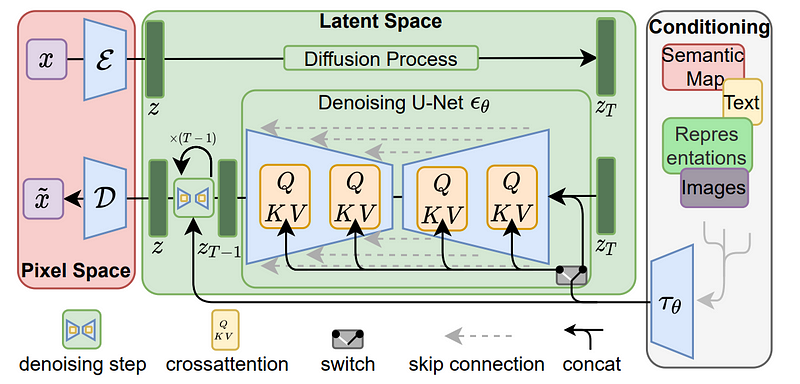
\includegraphics[width=0.8\textwidth]
{static/LDM.png}
\caption{The LDM \cite[Fig.~3]{Rombach_2022_CVPR}.}
\label{fig:ldm}
\end{figure}



\subsubsection{The Autoencoder}
A Variational Autoencoder (VAE) consists of two parts: the encoder and the decoder. "During latent diffusion training, the encoder is used to get the latent representations (latents) of the images for the forward diffusion process, which applies more and more noise at each step" \cite{patil2022stable}. The decoder conversely transforms the denoised latents, created by the U-Net, back into the pixel space at the end of the diffusion process. Only the decoder is used for the image generation process (see Fig.~\ref{fig:ldm}).



\subsubsection{The U-Net}
The U-Net \cite{ronneberger2015u} is a type of Convolutional Neural Network (CNN) that is responsible for predicting the noise in the current sample image. The image generation process starts with a random sample image of gaussian noise. The U-Net then takes this sample \((latents)\) and predicts the noise residual \((noise\_pred)\) of the image. 
This noise residual is partially \((sigma)\) removed in every step, until we end up with the final fully denoised image (see Fig.~\ref{fig:ldm}).
\begin{lstlisting}[language=Python]
latens = latents - sigma * noise_pred
\end{lstlisting}
The U-Net consists of an encoder and a decoder with transformer-based blocks. "Thus, it first encodes the current noised image as a set of tokens, then passes it through a series of transformer blocks" \cite{bolya2023tomesd}. The inclusion of transformer-based blocks allows the model to not only preserve the spacial hierarchies but also the semantic structure of the image.\\
A further aspect that distinguishes the U-Net from an autoencoder are the skip connections that directly pass information from the encoder to the decoder, aiding in the preservation of details during upsampling (see Fig.~\ref{fig:ldm}).



\subsubsection{The Text-Encoder}
The text-encoder is a transformer-based encoder that converts the input prompt from a string to an embedding vector that captures the semantic meaning of text and can be interpreted by the U-Net. Stable Diffusion uses CLIP's \cite{radford2021learning} pre-trained text-encoder \href{https://huggingface.co/docs/transformers/model_doc/clip#transformers.CLIPTextModel}{CLIPTextModel} and thus avoids additional training of the text-encoder.



\subsubsection{The Transformer Block}
Every transformer block has a self-attention (self-attn), cross-attention (cross-attn) and multi-layer perceptron (mlp) module.
The transformer also has residual connections around these modules to preserve important information and improve gradient flow, as well as multiple layer normalization blocks.



\subsubsection*{Self-Attention}
Self-attention \cite{vaswani2017attention} takes a series of (token) vectors and computes outputs while attending to every other token in the sequence.\\
The input vectors \((X)\) are firstly transformed into three different embedding matrices called Queries \((Q)\), Keys \((K)\) and Values \((V)\),  by multiplying the inputs with special transformation matrices \((W_Q, W_K, W_V)\). Then the self-attention module computes the attention weights \((A)\) for every pair of input vectors by taking the scaled dot-product of the Query and Key matrix and then applying the softmax-function. Lastly, the output vectors \((Y)\) are generated by taking a weighted sum of the Value embeddings with the attention weights (see Fig.~\ref{fig:self-attn}).\\
The output vectors are transformed representations of the input vectors, considering their interactions with every other input vector. The outputs are then passed on to the subsequent layers of the transformer. Self-attention enables the transformer to capture global dependencies in images or text.
\begin{figure}[!htb]
\centering
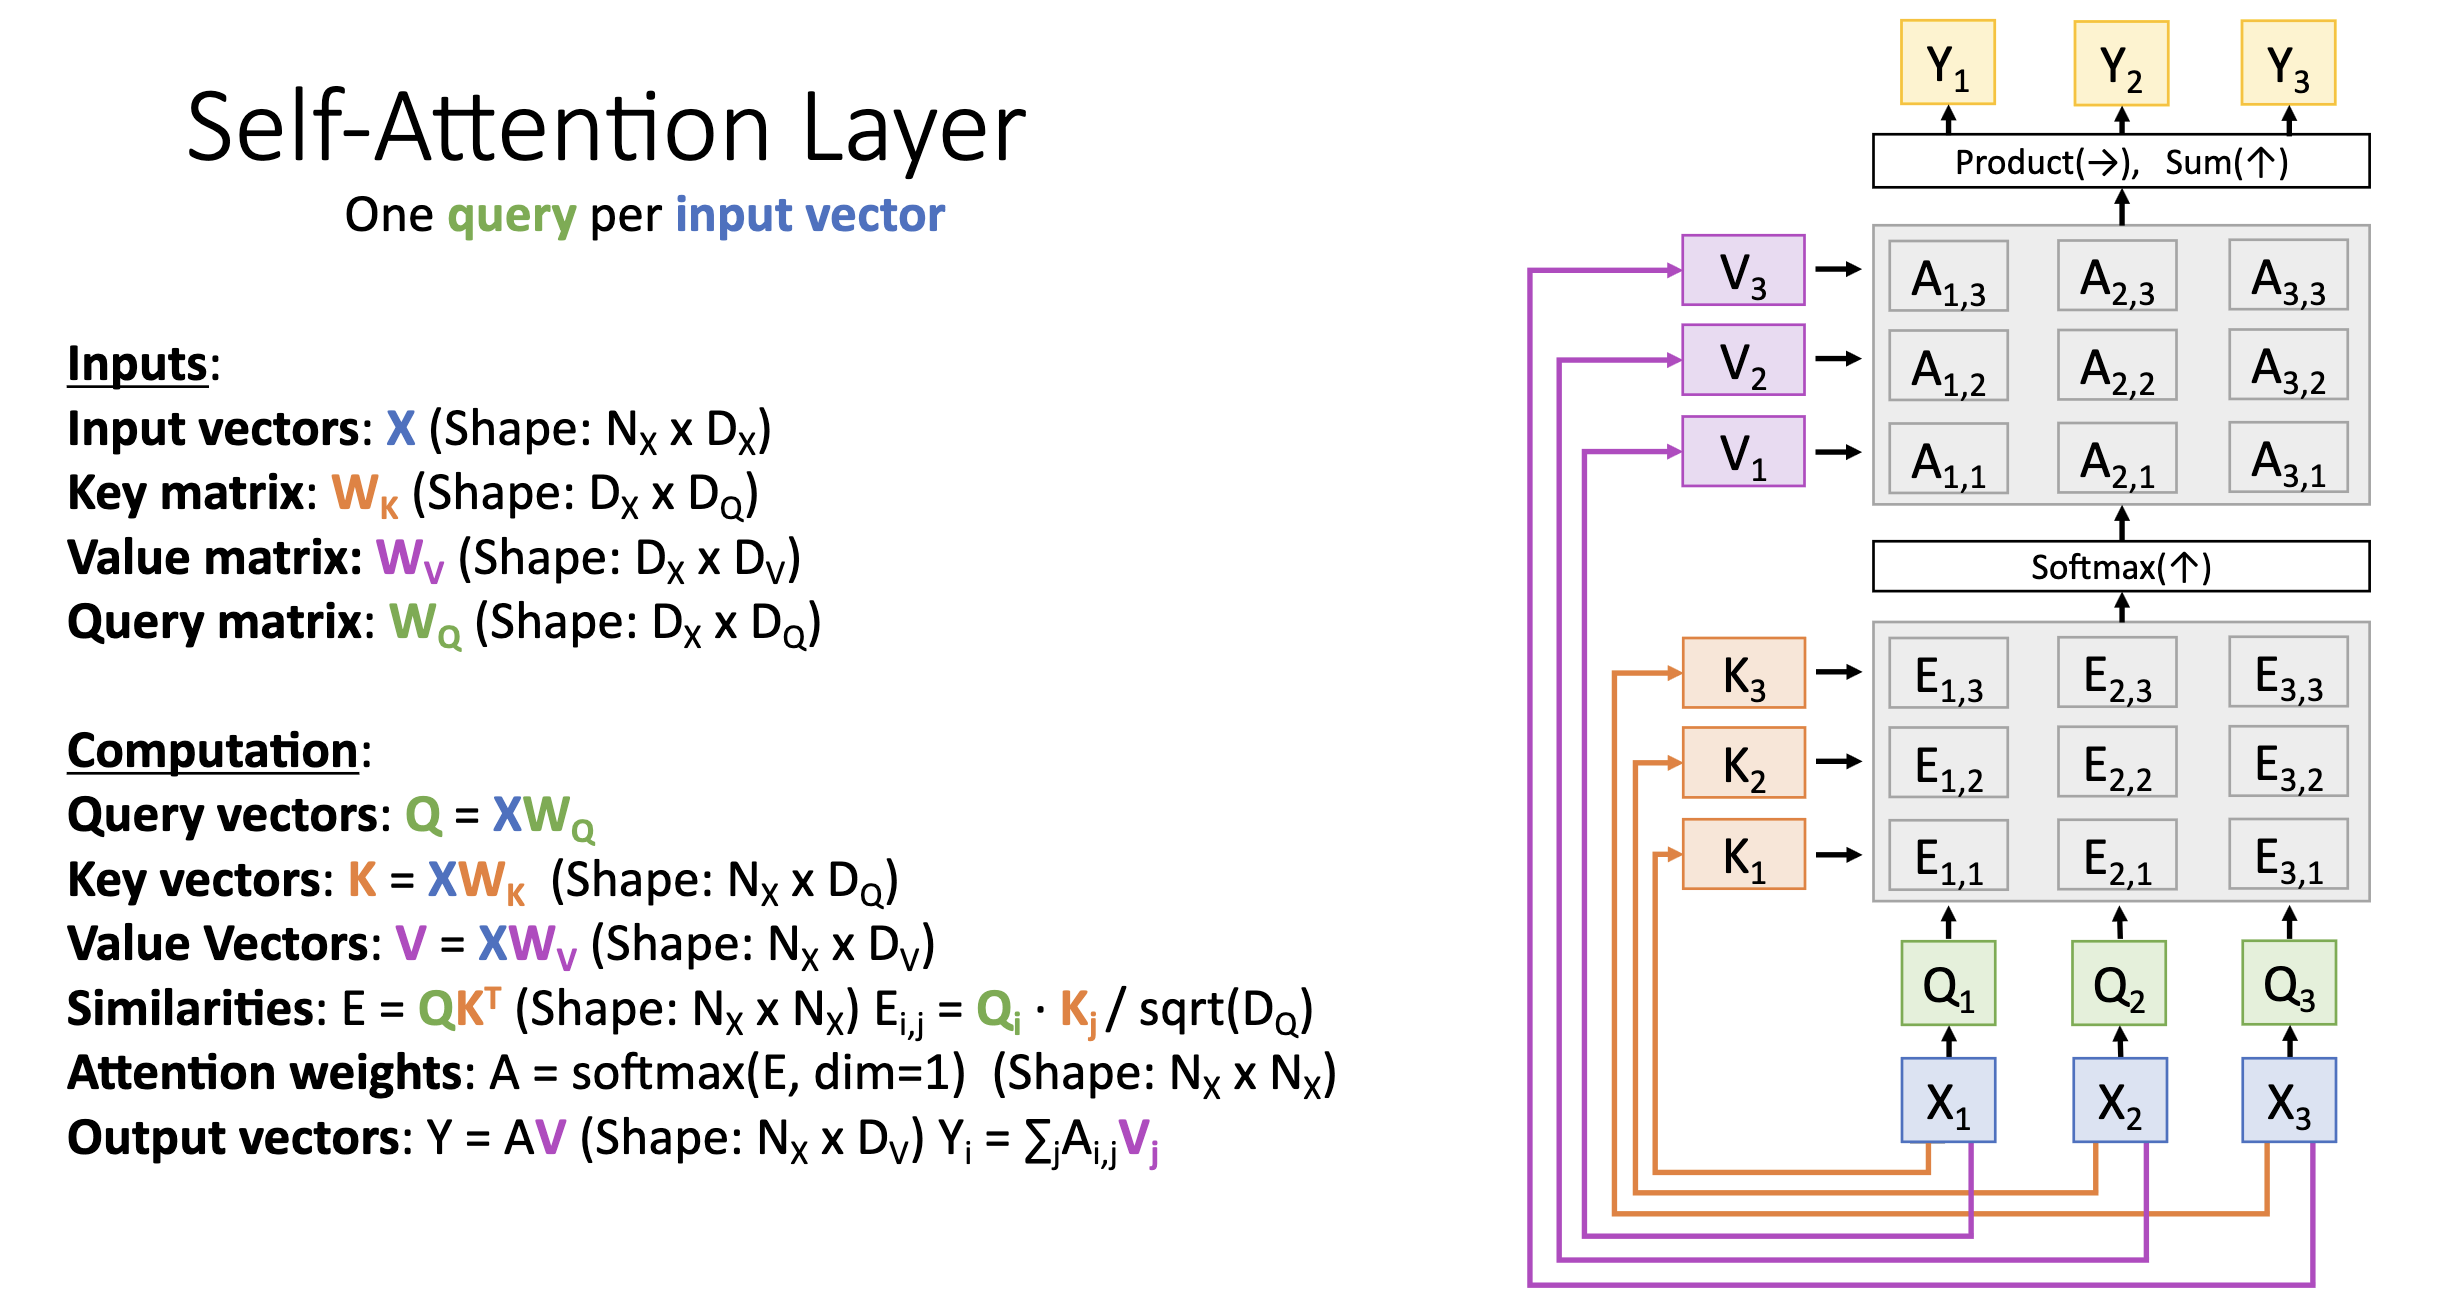
\includegraphics[width=0.95\textwidth]
{static/self_attn.png}
\caption{Self-attention \cite{johnson2019attn}}
\label{fig:self-attn}
\end{figure}



\subsubsection*{Cross-Attention}
Cross-attention creates its output from two input embeddings \((X_1, X_2)\) by generating \(Q\) from one input \((Q=X_1W_Q)\), and 
\(K\) and \(V\) from the other \((K=X_2W_K,\ V=X_2W_V)\). The algorithm is identical to self-attention from this point onwards.\\ Cross-Attention allows the model to consider both visual and semantic information when generating sequences, which enables the U-Net to attend to both the image and the prompt at the same time.



\subsubsection*{Multi-Layer Perceptron}
A multi-layer perceptron is a fully connected neural network. The mlp layer takes the outputs of the previous layer and applies an mlp network to each vector independently. This network consists of two linear transformations with a non-linear activation function (e.g., GELU \cite{hendrycks2016gaussian}) in between. Non-linearity exists exclusively in the mlp layer, allowing the transformer to capture more complex patterns in the data. It is particularly effective at modeling short-range patterns and local dependencies within a sequence.



\subsection{Fréchet-Inception-Distance}
The Fréchet Inception Distance (FID) is a metric that is used to evaluate the quality of generated images. It provides a quantitative measure of similarity by calculating the distance between the distributions of feature vectors of two image datasets. The feature vectors are extracted from the Inception model and the mean and covariance of their distributions are calculated.\\
"We call the Fréchet distance \(d(., .)\)
between the Gaussian with mean \((m, C)\) obtained from \(p(.)\) and the Gaussian with mean \((m_w, C_w)\)
obtained from \(p_w(.)\) the “Fréchet Inception Distance” (FID), which is given by:
\begin{align*}
    d^2((m,C),(m_w,C_w)) = || m - m_w ||_2^2 + Tr(C+C_w-2(CC_w)^\frac{1}{2})" 
\end{align*}
\cite{heusel2017gans}.\\
A lower FID value indicates greater similarity between the two image sets.



\subsubsection{Inception Model}
The Inception model \cite{Szegedy_2015_CVPR} is a deep convolutional neural network developed by Google researchers that is pretrained on ImageNet \cite{deng2009imagenet}. The model improves performance and efficiency in image classification and computer vision tasks by using multiple convolutional filter operations at different scales within the same layer.\\
The Inception model is used in the context of FID for creating low-dimensional latent representations of the input images, utilizing its ability to capture meaningful image features.
Current code implementations such as \cite{Seitzer2020FID} use the model's third iteration Inception-v3 \cite{szegedy2016rethinking}.



\subsubsection{Caveats}
FID is statistically biased, with its bias growing inversely proportional to the size of the image set, and the bias also depending on the model used for feature extraction \cite{Chong_2020_CVPR}. This makes comparing specific FID values from different experiments impossible, when identical sample sizes or the use of the same model are not guaranteed.\\
A further limitation of FID is the Inception model's compression of images to $299 \times 299$ pixels \cite{szegedy2016rethinking}. Thus, assessing the quality of larger images is additionally hindered as information about the images is lost by the compression.



\subsection{What are Tokens?}
Tokens are semantic units that can be processed by transformer-based models such as Stable Diffusion. Text, such as the prompt in image generation, is tokenized into words or subwords, which are then mapped to an embedding vector by the text-encoder. Image tokens capture discrete representations of their specific visual elements, with each token encoding a certain aspect of the image, such as a particular object, texture, color, or spatial region. This breakdown into smaller units is necessary for efficient computations and memory management, additionally enabling these algorithms to better capture patterns and relationships within the data.

%\newpage
\section{Related Work} \label{related_work}


\subsection{Token Pruning}
Several works have tried to utilize the transformer's flexibility when it comes to handling inconsistent amounts of tokens by pruning tokens that are considered the least important \cite{meng2022adavit,yin2022vit}. 
Differing from ToMe, these methods require model-specific training. Additionally, they dynamically determine the number of pruned tokens, resulting in variances between images. The flexibility in token number may improve accuracy, but makes batching of different samples impossible and requires the use of masks for training. This eradicates, or at least limits, the speedup that can be gained during training.\\
ToMe does not suffer from these problems as the number of tokens always stays the same outside of transformer components and generally no training is required. Still, ToMe achieves speedups in both image generation and training of models \cite{bolya2023tomesd}.



\subsection{Combining Tokens}
Other works try to combine tokens instead of pruning them.
There have been different approaches ranging from fusing less informative tokens into a single package token \cite{kong2021spvit, liang2022not}, over using a multi-layer perceptron with spatial attention for token reduction \cite{ryoo2021tokenlearner}, to using a learned deformable token merging module for adaptive token merging between stages \cite{pan2022less}.\\
The most similar method to ToMe is Token Pooling by \cite{marin2021token}, though it does again require specific finetuning. Token Pooling reduces the number of tokens to \(K\) by using k-means to cluster the tokens into \(K\) clusters. In this case the cluster centers represent the new tokens. The k-means-algorithm is slow, therefore Token Pooling offers a bad speed-accuracy trade-off.\\
ToMe is the only algorithm that offers reasonable speed and accuracy, without requiring any training \cite{bolya2023tome}.



%\subsection*{Efficient Transformers?}

\newpage
\section{Token Merging}
In Token Merging for Stable Diffusion (ToMe) by \cite{bolya2023tomesd}, the number of tokens in a transformer is reduced by \(r\)\% through merging similar tokens before every diffusion step and unmerging them afterward to retain the original size of the image.\\
The tokens are partitioned into a source (\textbf{src}) and a destination (\textbf{dst}) set, then the most similar tokens from the \textbf{src} set are continously merged into their \textbf{dst} counterparts until the number of tokens has reduced by \(r\)\%.\\
The choice of \(r\) is a trade-off between image fidelity and diffusion time as a lower amount of tokens requires a smaller computation time but more information about the image is lost in the merge process.\\
The merge can be applied in different components of the transformer (i.e., self-attn, cross-attn, mlp).



\subsection{Merge and Unmerge Algorithms}
\subsubsection*{Merging.} The Merge algorithm uses Bipartite-Soft-Matching to determine the similarity of tokens between the \textbf{src} and \textbf{dst} set. The two most similar tokens are taken and merged into a new token until the overall number of tokens has reduced by \(r\%\).\\
Two tokens \(x_1, x_2 \in \mathbb{R}^c\) would be merged into a new token \(x_{1,2}^* \in \mathbb{R}^c \), by averaging it's features: \[x_{1,2}^* = \frac{x_1 + x_2}{2}\]



\subsubsection*{Unmerging.} The Unmerge algorithm takes an originally merged token $x_{1,2}^* \in \mathbb{R}^c$ and splits it up into its original tokens $x_1', x_2' \in \mathbb{R}^c$: 
\begin{align*}
    x_1' = x_{1,2}^* \quad\quad
    x_2' = x_{1,2}^*
\end{align*}
in order to recreate the pre-merge amount of tokens.\\
This naive approach does lose information because the now unmerged tokens both have the average of their previous values, but this loss is small due their already high similarity before the merge.\\ Further exploration might yield improvements here.



\subsection{Bipartite-Soft-Matching}
Bipartite-Soft-Matching involves two main steps. First, the tensor of tokens is split into two tensors, one consisting of the \textbf{src} tokens and the other of \textbf{dst} tokens. Then, each token in the \textbf{src} set is matched with its most similar token in the \textbf{dst} set, creating a bipartite graph, with the edges between every \textbf{src} token and their closest match in the \textbf{dst} set. 



\subsubsection*{Choosing src and dst}
The grid of tokens is partitioned into a grid of \(sx \times sy\) batches of tokens.\\
Within every batch one token is chosen for the \textbf{dst} set with the rest now belonging to the \textbf{src} set. The choice is either random (default) or the top left token is always chosen when the parameter \textbf{use\_rand=False} is set.\\
\\
The number of mergeable tokens, which corresponds to the size of the \textbf{src} set, is limited by the choice of \(sx\) and \(sy\).
\begin{align*}
    r_{max} = 1-\frac{1}{sx*sy}
\end{align*}
That means for \(sx = 2\) and \(sy = 2\), no more than 75\% of tokens can be merged.\\
In the subsequent steps, the two most similar tokens are chosen greedily and merged into one, until \(r\%\) of tokens are gone.



\subsection{Token Similarity}
It is also relevant to define what "token similarity" exactly means. Bolya et al. explained: "While it may be tempting to call two tokens similar if the distance between their features is small, this is not necessarily optimal. The intermediate feature space in modern transformers is overparameterized. Luckily, transformers natively solve this problem with QKV self-attention \cite{vaswani2017attention}.\\
Specifically, the keys (K) already summarize the information contained in each token for use in dot product similarity. Thus, we use cosine similarity between the keys of each token to determine which contain similar information" \cite{bolya2023tome}.




%\newpage
\subsubsection*{Computing cosine similarity}
ToMe extracts the hidden states tensor (\(M\)) of the image and normalizes it before its \(split\) into two tensors (\(S\) and \(D\)), separating the \textbf{src} and \textbf{dst} tokens.
\begin{lstlisting}[language=Python]
M = M / M.norm(dim=-1, keepdim=True)
S, D = split(M)
\end{lstlisting}
Continuing from there, the cosine similarity (\(scores\)) between every \textbf{src} and \textbf{dst} token is computed by taking the dot product of \(S\) and \(D\).
\begin{lstlisting}[language=Python]
scores = S @ D.transpose(-1, -2)
\end{lstlisting}
The \(r\) most similar tokens of \textbf{src} and \textbf{dst} can now be identified by the indices of the largest values of the \(scores\) tensor.



\subsection{Additional Technical Information}
ToMe, in its basic form, only merges tokens in the self-attn block and defaults to using \(2 \times 2\) batches for token partitioning, with a randomly chosen \textbf{dst} token for every batch, resulting in a 75\% \textbf{src} and 25\% \textbf{dst} split. \\
ToMe is also not applied in every network block, but only the ones with the most tokens. Bolya and Hoffman argued:
"Applying ToMe to every block in the network is not ideal, since blocks at deeper U-Net scales have much fewer tokens. We try restricting ToMe to only blocks with some minimum number of tokens and find that only the blocks with the most tokens need ToMe applied to get most of the speed-up" \cite{bolya2023tomesd}.\\
Bolya and Hoffman also contemplated to scale the volume of token merging within the diffusion process of an image, but they concluded to keep the amount of tokens merged the same for every diffusion step, stating: "It might not be right to reduce the same number of tokens in each diffusion step. Earlier diffusion steps are coarser and thus might be more forgiving to errors. We test this by linearly interpolating the percent of tokens reduced and find that indeed merging more tokens earlier and fewer tokens later is slightly better, but not enough to be worth it" \cite{bolya2023tomesd}.

%\newpage
\section{Experimental Procedures}
We perform several experiments using the model "stable-diffusion-v1-5" by runwayml \cite{Rombach_2022_CVPR} and applying ToMe in different ways to a set of prompts and measuring the performance.
The performance is defined by\\ 
\(1)\) speed: the average diffusion time for every image of the set and\\
\(2)\) image quality: the FID-value between sets of images that had token merging applied and their counterparts (that is same prompt, seed and image size) that didn't use any token merging.



\subsection{Setup}
\subsubsection*{Creating image datasets}
The experiments always compare how diffusion time and image quality change across a spectrum of different volumes of tokens \((r)\) removed while token merging is applied in different layers of the transformer (self-attention, cross-attention and mlp).\\
The images were generated with a "DiffusionPipeline" from HuggingFace's diffusers library \cite{von-platen-etal-2022-diffusers}, using the "stable-diffusion-v1-5" model \cite{Rombach_2022_CVPR}.\\
We sampled multiple sets of \(n=500\) prompts from the dataset \href{https://huggingface.co/datasets/Gustavosta/Stable-Diffusion-Prompts}{Gustavosta/Stable-Diffusion-Prompts} on HuggingFace which has 80,000 prompts filtered and extracted from the image finder for Stable Diffusion: \href{https://lexica.art}{Lexica.art}, and generated a corresponding set of random seeds.\\ 
Prompts appearing multiple times within a set were not specifically prevented, due to the extremely low probability of a specific prompt-seed-pair appearing multiple times within a dataset. Same prompts with different seeds result in different images and therefore do not corrupt the validity of a dataset by our assessment.\\
Multiple images were created per prompt, with a 0\%, 10\%, 20\%, 30\%, 40\%, 50\%, and 60\% (if possible) merge applied respectively, creating a set of 3,500 (or sometimes 3,000) images which can be split up into subsets of 500 images each for every merge volume.\\
---cfg scale? number diffusion steps?---



\subsubsection*{Measuring results}
For image quality, FID between a subset with \(r > 0\%\) and the subset with \(r = 0\%\) of the same dataset is computed, to see how ToMe performs with different values for \(r\).\\
The speed of image generation is assessed by recording the time taken to create each individual image and then calculating the average across all subsets.
\begin{lstlisting}[language=Python]
start = time.time()
image = pipeline(prompt, x, y, ...)
end = time.time()
time = end - start
\end{lstlisting}



\subsubsection*{Hardware}
All experiments were conducted with Nvidia GeForce GTX 1080 Ti GPUs. Individual images were always created on a single GPU.



\subsection{Adjustments}
\subsubsection*{FID}
We created and used our own fork of pytorch-fid \cite{Seitzer2020FID} to accommodate for the hpc not being connected to the internet and therefore not being able to download the weights of the Inception model to calculate FID-values. Our fork loads these weights from a local directory to avoid any connection to the internet and requires the user to have them pre-installed.



\subsubsection*{Prompts}
We shortened every prompt that exceeds 300 characters, in order to ensure that CLIP's token limit is not breached, as CLIP can only handle up to 77 tokens.
This is done by determining the index (\(idx\)) of the last comma in the first 300 characters of every oversized prompt and then cutting off everything from this point onwards.
\begin{lstlisting}[language=Python]
prompt = prompt[:idx]
\end{lstlisting}


\newpage
\subsection{Comparison to Original Setup}
\cite{bolya2023tomesd} structure their experiments as follows: "We use Stable diffusion v1.5 to generate 2,000 $512 \times 512$ images of ImageNet-1k \cite{deng2009imagenet} classes (2 per class) using 50 PLMS \cite{liu2022pseudo} diffusion steps with a cfg scale \cite{dhariwal2021diffusion} of 7.5. We then compute FID scores between those 2,000 samples and 5,000 class-balanced ImageNet-1k val examples using \cite{Seitzer2020FID}. To test speed, we simply average the time taken over all 2,000 samples on a single 4090 GPU."\\
%\newpage
The most notable difference to our setup is that we compare a set of merged images with their own unmerged versions, while Bolya and Hoffman's approach compares image sets of the same categories but does not directly try to measure alterations of images created by ToMe.\\
Additionally, Bolya and Hoffman also measured and analyzed the memory usage during the diffusion process, we left memory consumption completely out of the scope of this work.



%\newpage
\subsection{Results}
The baseline is to look at the effects of ToMe (with default settings) applied to $768 \times 768$ images. The experiments can be split up into three different parts inspecting how ToMe affects performance\\ \(1)\) when applied to different parts of the transformer,\\ \(2)\) when applied to smaller $512 \times 512$ images, and\\ \(3)\) when different settings for partitioning the \textbf{src} and \textbf{dst} sets are used.\\
\\
The results of every experimental unit are presented in two figures. The first figure focuses on image quality, displaying FID values, while the subsequent one emphasizes image generation speed by showcasing how the average time required for image generation of each subset compares to the \(r=0\%\) subset.
Both figures have \(r\%\) on the x-axis showing how the metrics change with an increasing amount of tokens merged.

\subsubsection*{1): Experimenting with different components of the transformer}
ToMe's default configuration involves token merging solely within the self-attention module.
Our experiment aims to gauge how the performance metrics are affected by extending token merging to different combinations of transformer components.\\
All image sets were created with the same set of prompts and seeds (unless stated otherwise) to ensure the comparability of the results.



\subsubsection*{1.1): default (only self-attn) vs all (self-attn, cross-attn and mlp)}
The first experiment of part 1 compares the default setting of ToMe where token merging is only applied in the self-attn layer (black) with a different configuration that has token merging applied in the self-attn, cross-attn and mlp layer (red). 
The naive idea here is to improve performance by using token merging in every transformer layer.
\begin{figure}[!htb]
\label{fig:exp_1_1}
   % FID values for run2 and run3
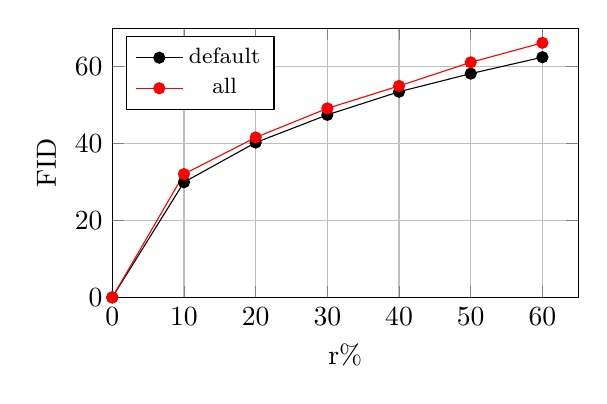
\begin{tikzpicture}
\begin{axis}[
    title={},
    height=5cm,
    width=7.5cm,
    xlabel={r\%},
    ylabel={FID},
    xmin=0, xmax=65,
    ymin=0, ymax=70,
    xtick={0,10,20,30,40,50,60},
    ytick={0,20,40,60},
    legend pos=north west,
    xmajorgrids=true,
    ymajorgrids=true,
    legend style={font=\footnotesize}
]

\addplot[
    color=black,
    mark=*
    ]
    coordinates {
    (0,0)(10,29.95)(20,40.26)(30,47.47)(40,53.48)(50,58.19)(60,62.46)
    };
    
\addplot[
    color=red,
    mark=*
    ]
    coordinates {
    (0,0)(10,32.07)(20,41.60)(30,49.15)(40,54.99)(50,61.13)(60,66.20)
    };
    
\legend{default, all}
    
\end{axis}
\end{tikzpicture}
   % time values for run2 and run3
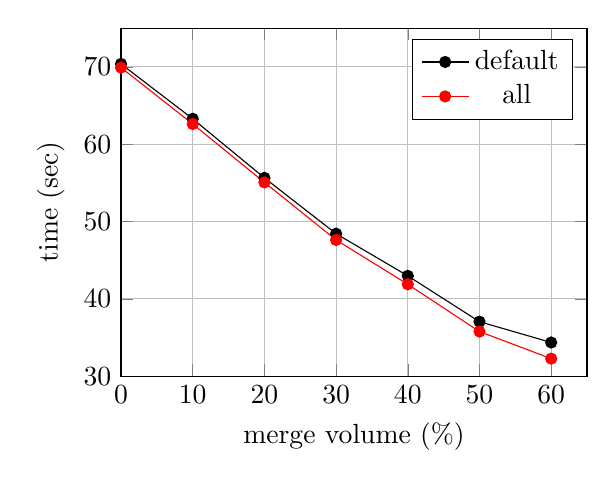
\begin{tikzpicture}
\begin{axis}[
    title={},
    height=6cm,
    width=7.5cm,
    xlabel={merge volume (\%)},
    ylabel={time (sec)},
    xmin=0, xmax=65,
    ymin=30, ymax=75,
    xtick={0,10,20,30,40,50,60},
    ytick={30,40,50,60,70},
    legend pos=north east,
    xmajorgrids=true,
    ymajorgrids=true,
]

\addplot[
    color=black,
    mark=*
    ]
    coordinates {
    (0,70.38)(10,63.28)(20,55.64)(30,48.42)(40,42.97)(50,37.04)(60,34.35)
    };
    
\addplot[
    color=red,
    mark=*
    ]
    coordinates {
    (0,69.91)(10,62.61)(20,55.06)(30,47.61)(40,41.88)(50,35.76)(60,32.26)
    };
    
\legend{default, all}
    
\end{axis}
\end{tikzpicture}
\caption{FID and relative time compared to r=0\% for 1.1)}
\label{fig:exp_1_1}
\end{figure}\\
%\newpage
This seemingly does not yield significant improvements as image generation speed does narrowly decrease by up to 2.1 s/im (this time-delta is below 1 s/im for $r<40\%$ though; see Tab.~\ref{table:exp_1_1}), albeit at a clear cost of image quality with FID being consistently larger for this configuration. \\
ToMe in its default setup consistently produces images closer to their no-ToMe original (see Fig.~\ref{fig:exp_1_1}), so extending token merging to both the cross-attn and mlp layer does not appear beneficial. This naive approach can therefore be disregarded.



%\newpage
\subsubsection*{1.2): [default] vs [self-attn \& cross-attn] vs [self-attn \& mlp]}
After \(1.1\), the question remains whether performance drops were caused by using ToMe in both the cross-attn and mlp layer or only one of them, so the second experiment of part 1 attempts to delve deeper into that matter. This time token merging is only extended to either the cross-attn (red) or the mlp module (blue). Then a comparison is made with the results of the default ToMe settings (black) from the previous trial.
\begin{figure}[!htb]
    % FID values for run2, run4 and run5
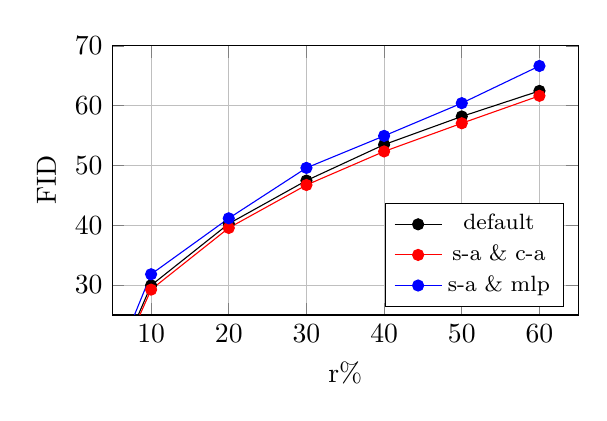
\begin{tikzpicture}
\begin{axis}[
    title={},
    height=5cm,
    width=7.5cm,
    xlabel={r\%},
    ylabel={FID},
    xmin=5, xmax=65,
    ymin=25, ymax=70,
    xtick={10,20,30,40,50,60},
    ytick={30,40,50,60,70},
    legend pos=south east,
    xmajorgrids=true,
    ymajorgrids=true,
    legend style={font=\footnotesize}
]

\addplot[
    color=black,
    mark=*
    ]
    coordinates {
    (0,0)(10,29.95)(20,40.26)(30,47.47)(40,53.48)(50,58.19)(60,62.46)
    };
    
\addplot[
    color=red,
    mark=*
    ]
    coordinates {
    (0,0)(10,29.24)(20,39.55)(30,46.73)(40,52.34)(50,57.05)(60,61.64)
    };

\addplot[
    color=blue,
    mark=*
    ]
    coordinates {
    (0,0)(10,31.81)(20,41.16)(30,49.59)(40,54.94)(50,60.41)(60,66.63)
    };
    
\legend{default, s-a \& c-a, s-a \& mlp}
    
\end{axis}
\end{tikzpicture}
    % time values for run2, run4 and run5
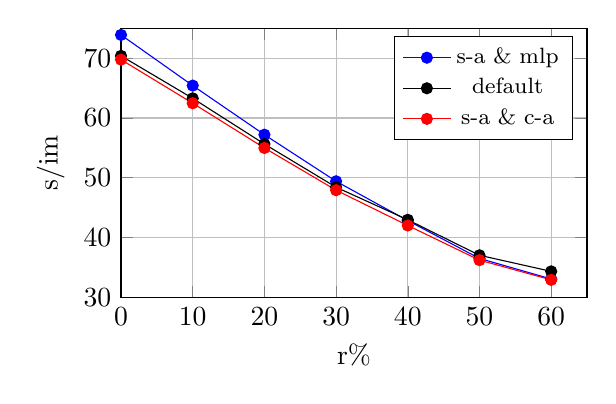
\begin{tikzpicture}
\begin{axis}[
    title={},
    height=5cm,
    width=7.5cm,
    xlabel={r\%},
    ylabel={s/im},
    xmin=0, xmax=65,
    ymin=30, ymax=75,
    xtick={0,10,20,30,40,50,60},
    ytick={30,40,50,60,70},
    legend pos=north east,
    xmajorgrids=true,
    ymajorgrids=true,
    legend style={font=\footnotesize}
]

\addplot[
    color=blue,
    mark=*
    ]
    coordinates {
    (0,73.88)(10,65.41)(20,57.20)(30,49.41)(40,42.83)(50,36.51)(60,33.08)
    };

\addplot[
    color=black,
    mark=*
    ]
    coordinates {
    (0,70.38)(10,63.28)(20,55.64)(30,48.42)(40,42.97)(50,37.04)(60,34.35)
    };
    
\addplot[
    color=red,
    mark=*
    ]
    coordinates {
    (0,69.75)(10,62.46)(20,54.98)(30,47.92)(40,42.02)(50,36.23)(60,32.93)
    };

    
\legend{s-a \& mlp, default, s-a \& c-a}
    
\end{axis}
\end{tikzpicture}
\caption{FID and relative time compared to r=0\% for 1.2)}
\label{fig:exp_1_2}
\end{figure}\\
%\newpage
This time it's clearly visible that merging tokens within the self-attn and cross-attn module performs the best, both in terms of image quality and image generation speed, notably surpassing the default configuration established by Bolya and Hofmann (see Fig.~\ref{fig:exp_1_2}).\\
Token merging in the self-attn and mlp module on the other hand noticeably worsens the image quality across the board as well as the generation speed when $r<40\%$ compared to the default (see Tab.~\ref{table:exp_1_2}).\\
We can therefore conclude that extending token merging to the cross-attn module has positive effects on the performance, while extending it to the mlp module has the opposite effect.



%\newpage
\subsubsection*{1.3): [default] vs [cross-attn \& mlp] vs [only cross-attn]}
The common denominator of the previous examinations was the application of token merging in the self-attn layer. This time we are explicitly avoiding token merging in the self-attn module and instead apply it in only the cross-attn (blue) and both the cross-attn and mlp component (red).
The results of the default ToMe settings (black) again carry over from the previous trial.\\
\begin{figure}[!htb]
    % FID values for run2, run6 and run7
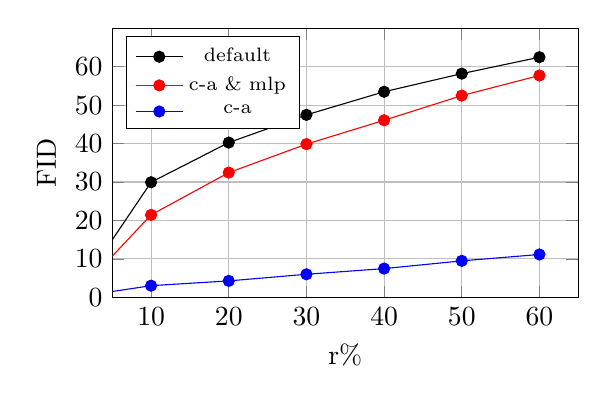
\begin{tikzpicture}
\begin{axis}[
    title={},
    height=5cm,
    width=7.5cm,
    xlabel={r\%},
    ylabel={FID},
    xmin=5, xmax=65,
    ymin=0, ymax=70,
    xtick={10,20,30,40,50,60},
    ytick={0,10,20,30,40,50,60},
    legend pos=north west,
    xmajorgrids=true,
    ymajorgrids=true,
    legend style={font=\scriptsize}
]

\addplot[
    color=black,
    mark=*
    ]
    coordinates {
    (0,0)(10,29.95)(20,40.26)(30,47.47)(40,53.48)(50,58.19)(60,62.46)
    };
    
\addplot[
    color=red,
    mark=*
    ]
    coordinates {
    (0,0)(10,21.46)(20,32.45)(30,39.86)(40,46.06)(50,52.48)(60,57.71)
    };

\addplot[
    color=blue,
    mark=*
    ]
    coordinates {
    (0,0)(10,3.05)(20,4.29)(30,6.01)(40,7.49)(50,9.50)(60,11.16)
    };

    
\legend{default, c-a \& mlp, c-a}
    
\end{axis}
\end{tikzpicture}
    % time values for run10 and run11
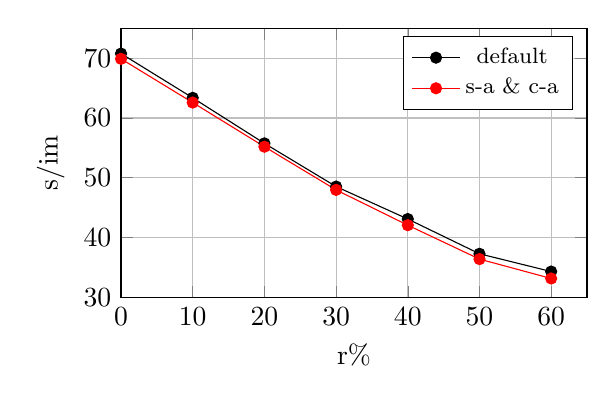
\begin{tikzpicture}
\begin{axis}[
    title={},
    height=5cm,
    width=7.5cm,
    xlabel={r\%},
    ylabel={s/im},
    xmin=0, xmax=65,
    ymin=30, ymax=75,
    xtick={0,10,20,30,40,50,60},
    ytick={30,40,50,60,70},
    legend pos=north east,
    xmajorgrids=true,
    ymajorgrids=true,
    legend style={font=\footnotesize}
]

\addplot[
    color=black,
    mark=*
    ]
    coordinates {
    (0,70.76)(10,63.36)(20,55.75)(30,48.53)(40,43.10)(50,37.29)(60,34.32)
    };
    
\addplot[
    color=red,
    mark=*
    ]
    coordinates {
    (0,69.88)(10,62.57)(20,55.19)(30,47.97)(40,42.07)(50,36.40)(60,33.16)
    };
    
\legend{default, s-a \& c-a}
    
\end{axis}
\end{tikzpicture}
\caption{FID and relative time compared to r=0\% for 1.3)}
\label{fig:exp_1_3}
\end{figure}\\
The most striking result here is that no token merging in the self-attn layer corresponds to no image generation speedup at all, rather slowing the process down (see Tab.~\ref{table:exp_1_3}). 
The apparent improvements to image quality compared to the ToMe default (see Fig.~\ref{fig:exp_1_3}) consequently become negligible without any speed benefits, though it can be noted that token merging in only the cross-attn layer greatly outperforms token merging in both cross-attn and mlp layer in terms of image quality.\\
We conclusively derive that ToMe without involvement of the self-attn layer does not accelerate the image generation process at all and can be considered redundant and therefore be disregarded. It can additionally be derived from \(1.1 - 1.3\) that token merging in the mlp layer has strong negative effects on image quality.




%\newpage
\subsubsection*{1.4): [default] vs [self-attn \& cross-attn] (the second time)}
The most prominent takeaway of the first three experiments is that token merging in both the self-attn and cross-attn layers improves the performance of ToMe both in terms of image quality and image generation speed.\\
We want to further examine this discovery by repeating the experiment with a new set of 500 different prompt-seed pairs and then average the results of both trials.
\begin{figure}[!htb]
    % FID values for run8 and run9
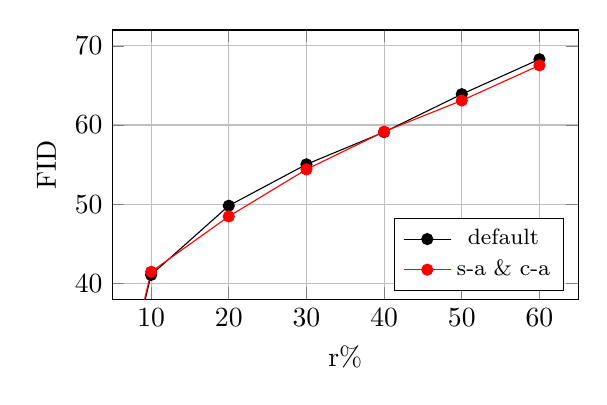
\begin{tikzpicture}
\begin{axis}[
    title={},
    height=5cm,
    width=7.5cm,
    xlabel={r\%},
    ylabel={FID},
    xmin=5, xmax=65,
    ymin=38, ymax=72,
    xtick={10,20,30,40,50,60},
    ytick={30,40,50,60,70},
    legend pos=south east,
    xmajorgrids=true,
    ymajorgrids=true,
    legend style={font=\footnotesize}
]

\addplot[
    color=black,
    mark=*
    ]
    coordinates {
    (0,0)(10,41.06)(20,49.80)(30,55.03)(40,59.10)(50,63.89)(60,68.30)
    };
    
\addplot[
    color=red,
    mark=*
    ]
    coordinates {
    (0,0)(10,41.45)(20,48.45)(30,54.39)(40,59.16)(50,63.09)(60,67.53)
    };
    
\legend{default, s-a \& c-a}
    
\end{axis}
\end{tikzpicture}
    % time values for run8 and run9
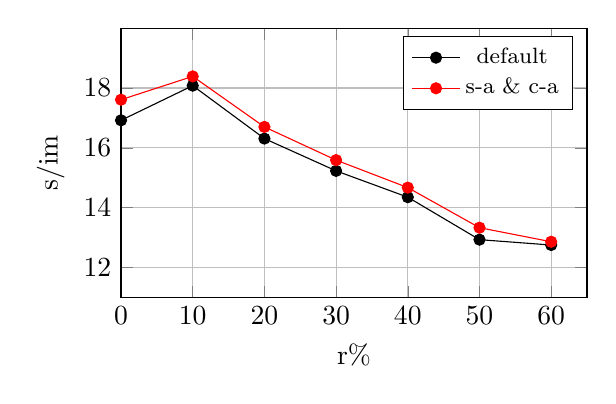
\begin{tikzpicture}
\begin{axis}[
    title={},
    height=5cm,
    width=7.5cm,
    xlabel={r\%},
    ylabel={s/im},
    xmin=0, xmax=65,
    ymin=11, ymax=20,
    xtick={0,10,20,30,40,50,60},
    ytick={12,14,16,18},
    legend pos=north east,
    xmajorgrids=true,
    ymajorgrids=true,
    legend style={font=\footnotesize}
]

\addplot[
    color=black,
    mark=*
    ]
    coordinates {
    (0,16.92)(10,18.08)(20,16.31)(30,15.23)(40,14.35)(50,12.93)(60,12.75)
    };
    
\addplot[
    color=red,
    mark=*
    ]
    coordinates {
    (0,17.61)(10,18.39)(20,16.70)(30,15.59)(40,14.67)(50,13.33)(60,12.86)
    };
    
\legend{default, s-a \& c-a}
    
\end{axis}
\end{tikzpicture}
\caption{FID and relative time compared to r=0\% for 1.4)}
\label{fig:exp_1_4}
\end{figure}\\
%\newpage
It is again clearly visible that token merging only in the self-attn module (black) is outperformed by expanding it to the cross-attn module (red) as well (see Fig.~\ref{fig:exp_1_4}). This improvement consistently appears with every \(r\), with the gap slightly widening for larger values of \(r\) (see Tab.~\ref{table:exp_1_4}).\\
This motivates the use of token merging in both the self-attn and cross-attn modules as the new default for $768 \times 768$ images going forward.



%\newpage
\subsubsection*{2): Exploring smaller images sizes}
In this section, we want to expand the scope of our trials to smaller image sizes. Precisely, we want to repeat looking at token merging in the self-attn layer (black) and both the self-attn and cross-attn layer (red), but this time with smaller $512 \times 512$ images. Again a set of 500 prompts is randomly sampled and a corresponding set of random seeds is generated.
\begin{figure}[!htb]
    % FID values for run8 and run9
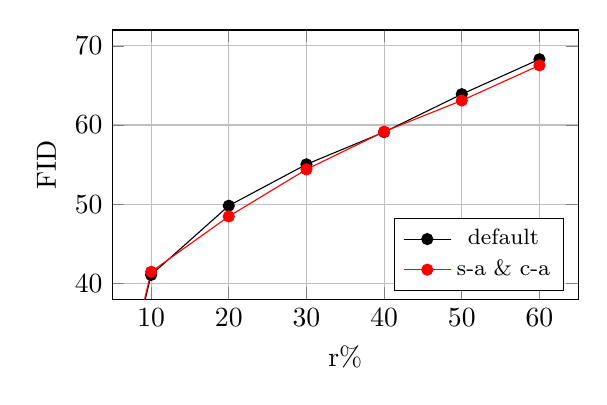
\begin{tikzpicture}
\begin{axis}[
    title={},
    height=5cm,
    width=7.5cm,
    xlabel={r\%},
    ylabel={FID},
    xmin=5, xmax=65,
    ymin=38, ymax=72,
    xtick={10,20,30,40,50,60},
    ytick={30,40,50,60,70},
    legend pos=south east,
    xmajorgrids=true,
    ymajorgrids=true,
    legend style={font=\footnotesize}
]

\addplot[
    color=black,
    mark=*
    ]
    coordinates {
    (0,0)(10,41.06)(20,49.80)(30,55.03)(40,59.10)(50,63.89)(60,68.30)
    };
    
\addplot[
    color=red,
    mark=*
    ]
    coordinates {
    (0,0)(10,41.45)(20,48.45)(30,54.39)(40,59.16)(50,63.09)(60,67.53)
    };
    
\legend{default, s-a \& c-a}
    
\end{axis}
\end{tikzpicture}
    % time values for run2, run6 and run7
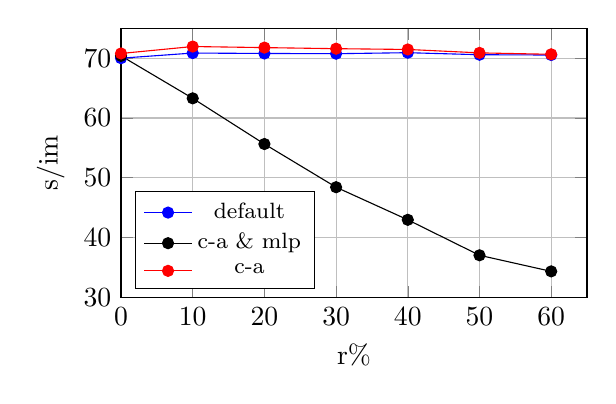
\begin{tikzpicture}
\begin{axis}[
    title={},
    height=5cm,
    width=7.5cm,
    xlabel={r\%},
    ylabel={s/im},
    xmin=0, xmax=65,
    ymin=30, ymax=75,
    xtick={0,10,20,30,40,50,60},
    ytick={30,40,50,60,70},
    legend pos=south west,
    xmajorgrids=true,
    ymajorgrids=true,
    legend style={font=\footnotesize}
]

\addplot[
    color=blue,
    mark=*
    ]
    coordinates {
    (0,69.99)(10,70.85)(20,70.78)(30,70.74)(40,70.91)(50,70.57)(60,70.52)
    };

\addplot[
    color=black,
    mark=*
    ]
    coordinates {
    (0,70.38)(10,63.28)(20,55.64)(30,48.42)(40,42.97)(50,37.04)(60,34.35)
    };
    
\addplot[
    color=red,
    mark=*
    ]
    coordinates {
    (0,70.78)(10,71.94)(20,71.76)(30,71.58)(40,71.45)(50,70.88)(60,70.64)
    };

    
\legend{default, c-a \& mlp, c-a}
    
\end{axis}
\end{tikzpicture}
\caption{FID and relative time compared to r=0\% for 2)}
\label{fig:exp_2}
\end{figure}\\
%\newpage
The success of \(1.4\) does not repeat, as this time it was consistently slower to create images with token merging in the cross-attn block (see Fig.~\ref{fig:exp_2}). The FID seems to bounce a bit with the default performing slightly better for \(r=10\%\) and \(r=40\%\), but performing worse the rest of the time (see Tab.~\ref{table:exp_2}). \\
The overall speed gains are considerably smaller compared to the \(768 \times 768\) images. Even at \(r=60\%\), the speed gain is only about 25\% and the image generation process actually becomes slower by about 1 s/im at \(r=10\%\) (see Tab.~\ref{table:exp_2}).\\
We conclude that using ToMe for such small images (e.g. $512 \times 512$ or smaller) is less practical than it is for larger images. It is especially inadvisable to be used with a small merge volume (\(r<20\%\)), as there is no time gained in the diffusion process, but information is nonetheless lost during merging. \\
In consequence, we will not investigate the usage of ToMe on this scale any further. Neither will we investigate ToMe's effect on larger images due to hardware limitations.



%\newpage
\subsubsection*{3): Exploring different batch sizes}
The third part of the experimental section examines, how different values for \(sx\) and \(sy\) influence the performance of ToMe on $768 \times 768$ images. As a reminder, \(sx\) and \(sy\) determine the size of the token batches, which are used to spread the \textbf{dst} tokens somewhat evenly across the image, with larger batches resulting in a less consistent distribution. Our new default of ToMe with token merging applied in both the self-attn and cross-attn layer will be used throughout this section.



%\newpage
\subsubsection*{3.1): $3 \times 3$ batches}
The first choice was scaling up from $2 \times 2$ (black) to $3 \times 3$ batches (red). This setup strongly tilts the ratio of src and dst tokens toward the former and theoretically allows for a larger number of tokens to be merged. 
\begin{align*}
    r_{max} = 1-\frac{1}{3*3} = \frac{8}{9} \approx 88.89\%
\end{align*}
We will, nevertheless, not exceed a merge rate of \(r=60\%\), as image quality already exhibits clear deterioration at that level and also due to the absence of other data available for comparison.



\subsubsection*{3.2): $1 \times 2$ vertical batches}
Scaling down the same way to $1 \times 1$ batches is impossible, as it would result in every token landing in the \textbf{dst} set and \(r_{max}=0\%\).\\
We therefore chose to cut the batches in half horizontally, creating $1 \times 2$ batches. This decision led to a balanced 50-50 distribution between \textbf{src} and \textbf{dst}.
\begin{align*}
    r_{max} = 1-\frac{1}{1*2} = 50\%
\end{align*}
This limits our merge volume to 50\% but allows for better matches during the merge process. Compared to the $2 \times 2$ default, every \textbf{src} token now has double the number of \textbf{dst} tokens to be matched with.\\
\begin{figure}[!htb]
    % FID values for run11, run14 and run15 
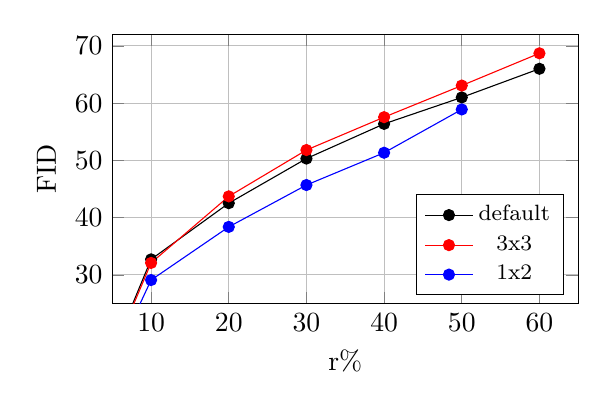
\begin{tikzpicture}
\begin{axis}[
    title={},
    height=5cm,
    width=7.5cm,
    xlabel={r\%},
    ylabel={FID},
    xmin=5, xmax=65,
    ymin=25, ymax=72,
    xtick={10,20,30,40,50,60},
    ytick={30,40,50,60,70},
    legend pos=south east,
    xmajorgrids=true,
    ymajorgrids=true,
    legend style={font=\footnotesize}
]

\addplot[
    color=black,
    mark=*
    ]
    coordinates {
    (0,0)(10,32.71)(20,42.52)(30,50.31)(40,56.37)(50,60.99)(60,65.99)
    };
    
\addplot[
    color=red,
    mark=*
    ]
    coordinates {
    (0,0)(10,32.09)(20,43.71)(30,51.80)(40,57.54)(50,63.06)(60,68.69)
    };

\addplot[
    color=blue,
    mark=*
    ]
    coordinates {
    (0,0)(10,29.10)(20,38.38)(30,45.69)(40,51.33)(50,58.89)
    };
    
\legend{default, 3x3, 1x2}
    
\end{axis}
\end{tikzpicture}
    % time values for run11, run14 and run15
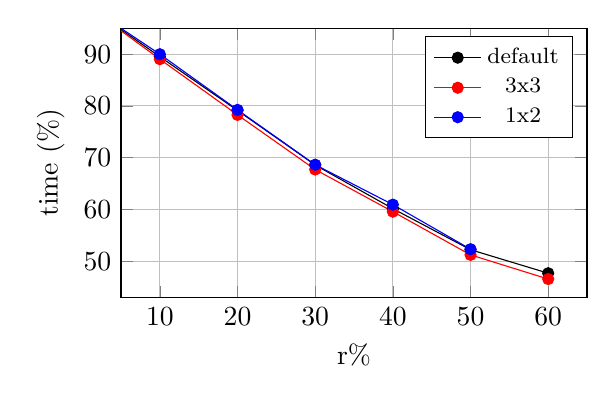
\begin{tikzpicture}
\begin{axis}[
    title={},
    height=5cm,
    width=7.5cm,
    xlabel={r\%},
    ylabel={time (\%)},
    xmin=5, xmax=65,
    ymin=43, ymax=95,
    xtick={10,20,30,40,50,60},
    ytick={50,60,70,80,90},
    legend pos=north east,
    xmajorgrids=true,
    ymajorgrids=true,
    legend style={font=\footnotesize}
]

\addplot[
    color=black,
    mark=*
    ]
    coordinates {
    (0,100)(10,89.50)(20,79.11)(30,68.57)(40,60.14)(50,52.21)(60,47.67)
    };
    
\addplot[
    color=red,
    mark=*
    ]
    coordinates {
    (0,100)(10,89.02)(20,78.26)(30,67.70)(40,59.56)(50,51.21)(60,46.54)
    };

\addplot[
    color=blue,
    mark=*
    ]
    coordinates {
    (0,100)(10,89.98)(20,79.23)(30,68.63)(40,60.92)(50,52.31)
    };
    
\legend{default, 3x3, 1x2}
    
\end{axis}
\end{tikzpicture}
\caption{FID and relative time compared to r=0\% for 3)}
\label{fig:exp_3}
\end{figure}\\
The resizing of the batches has only minor effects on image generation speed, as all three configurations consistently remain within one second of each other (see Tab.~\ref{table:exp_3}).\\
Image quality shows a noticeable improvement with decreasing batch sizes. The ToMe version with $3 \times 3$ batches is slightly surpassed by the $2 \times 2$ version, and this improvement is further enhanced when transitioning to $1 \times 2$ batches. (see Fig.~\ref{fig:exp_3}).
The gap closes towards \(r=50\%=r_{max}\), as every \textbf{src} token has to be merged when using $1 \times 2$ batches, regardless of how good of a match from \textbf{dst} is available.\\
It can still be concluded that using the $1 \times 2$ batches to create an equal number of \textbf{src} and \textbf{dst} tokens yields the best performance, especially when \(r\) is not close to \(0\%\) or \(r_{max}\), while the usage of larger batches with a smaller \(\textbf{dst\%}\) is not advisable.



%\newpage
\subsubsection*{4): Putting it all together}
Finally, we are comparing the most successful configurations from the past experiments. That means we are looking at \textbf{setup 1}: the ToMe default by Bolya and Hofmann (black), \textbf{setup 2}: our new default with token merging expanded to the cross-attn layer from \(1.2\) and \(1.4\) (red), and \textbf{setup 3}: the new default but with $1 \times 2$ batches for token partitioning from \(3.2\) (blue).\\
We expanded the image sets for the first two configurations to 1000 images per merge volume in \(1.4\), so we will do the same for the other one to enable examinations on a larger scale.
\begin{figure}[!htb]
    % FID values for run2/10, run4/11 and run15/16
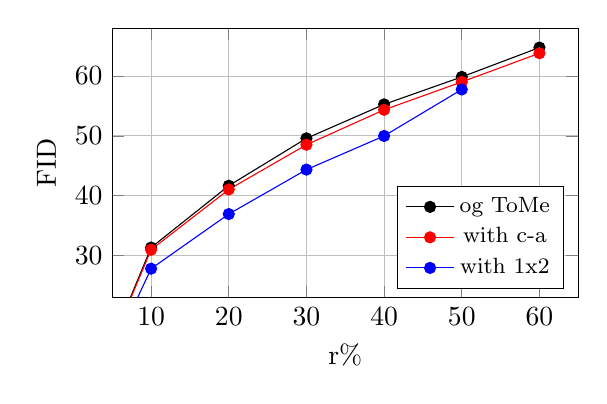
\begin{tikzpicture}
\begin{axis}[
    title={},
    height=5cm,
    width=7.5cm,
    xlabel={r\%},
    ylabel={FID},
    xmin=5, xmax=65,
    ymin=23, ymax=68,
    xtick={10,20,30,40,50,60},
    ytick={30,40,50,60},
    legend pos=south east,
    xmajorgrids=true,
    ymajorgrids=true,
    legend style={font=\footnotesize}
]

\addplot[
    color=black,
    mark=*
    ]
    coordinates {
    (0,0)(10,31.33)(20,41.67)(30,49.59)(40,55.27)(50,59.86)(60,64.77)
    };
    
\addplot[
    color=red,
    mark=*
    ]
    coordinates {
    (0,0)(10,30.97)(20,41.04)(30,48.52)(40,54.36)(50,59.02)(60,63.82)
    };

\addplot[
    color=blue,
    mark=*
    ]
    coordinates {
    (0,0)(10,27.80)(20,36.93)(30,44.36)(40,49.99)(50,57.76)
    };
    
\legend{og ToMe, with c-a, with 1x2}
    
\end{axis}
\end{tikzpicture}
    % time values for run2/10, run4/11, run15/16
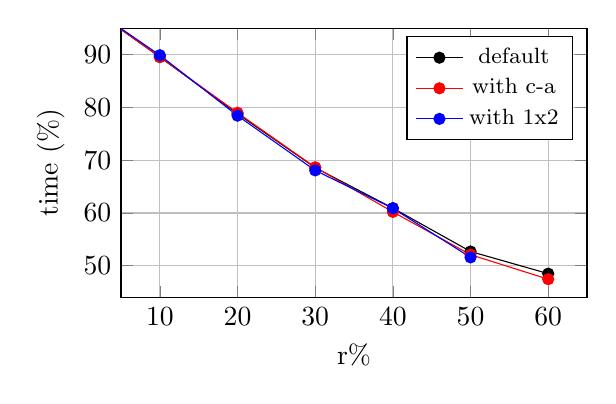
\begin{tikzpicture}
\begin{axis}[
    title={},
    height=5cm,
    width=7.5cm,
    xlabel={r\%},
    ylabel={time (\%)},
    xmin=5, xmax=65,
    ymin=44, ymax=95,
    xtick={10,20,30,40,50,60},
    ytick={50,60,70,80,90},
    legend pos=north east,
    xmajorgrids=true,
    ymajorgrids=true,
    legend style={font=\footnotesize}
]

\addplot[
    color=black,
    mark=*
    ]
    coordinates {
    (0,100)(10,89.54)(20,78.79)(30,68.58)(40,60.91)(50,52.70)(60,48.50)
    };
    
\addplot[
    color=red,
    mark=*
    ]
    coordinates {
    (0,100)(10,89.54)(20,78.98)(30,68.65)(40,60.20)(50,52.09)(60,47.45)
    };

\addplot[
    color=blue,
    mark=*
    ]
    coordinates {
    (0,100)(10,89.89)(20,78.43)(30,68.06)(40,60.88)(50,51.58)
    };
    
\legend{default, with c-a, with 1x2}
    
\end{axis}
\end{tikzpicture}
\caption{FID and relative time compared to r=0\% for 4)}
\label{fig:exp_4}
\end{figure}\\
Again, speed is very close across the board, as \textbf{setup 2} is the fastest by only a small margin (see Tab.~\ref{table:exp_4}).
Our discoveries regarding image quality are also reinforced, with \textbf{setup 3} noticeably outperforming the rest and \textbf{setup 1} consistently being the worst (see Fig.~\ref{fig:exp_4}).\\



%\newpage
\subsubsection*{Summary}
The experiments we conducted suggest that the best performance can be achieved by applying token merging in both the self-attn and cross-attn layer of the transformer. Depending on whether speed or image quality is the most important demand, $1 \times 2$ (best image quality) or $2 \times 2$ batches (highest speed) can be chosen for token partitioning, with $1 \times 2$ batches bringing particularly great improvements to image quality when \(r\leq40\%\).\\
Another important discovery is that token merging in the self-attn module is essential to unlocking speed improvements for image generation. On the other hand, using ToMe in the mlp layer seems to exclusively come at a disadvantage.\\
Moreover, it is important to create sufficiently large images when using ToMe in order to see the speed benefits. We showed that the time improvements with token merging noticeably decrease from >50\% for $768 \times 768$ images to only about 25\% for $512 \times 512$ images at \(r=60\%\) (see Tab.~\ref{table:exp_1_4},~\ref{table:exp_2}).\\
Additionally, it was shown that strongly skewing the \textbf{src}-\textbf{dst}-ratio away from an equal distribution has negative effects on image quality as well (see Tab.~\ref{table:exp_2}).




%\newpage
\subsection{Comparison to Original Results}
--Effects generally confirmed---
--Difference in details--
---1x2 grid performance gains contradict paper---
Note that FID doesn’t consider prompt adherence, which is likely why merging the cross-attn module actually reduces FID. (Still relevent with different expermient setup??)

%\newpage
\section{Further Exploration}
The results of our experiments could be improved by expanding research on the influence of different elements of ToMe's or SD's configuration.\\ 
The larger $768 \times 768$ images benefited noticeably more from token merging than the $512 \times 512$ images, so exploration whether this positive effect further scales up with image size could become relevant.\\
Another aspect we rather briefly touched upon is the selection of \textbf{dst} tokens. ToMe currently only selects one \textbf{dst} token per batch so experimenting with multiple \textbf{dst} tokens per batch and differently sized bacthes might improve performance as well.\\ 
Bolya and Hofmann also mentioned that further improvements could also be achieved by exploring better unmerging strategies or whether proportional attention or key-based similarity are useful for diffusion.
The current unmerge algorithm is quite naive, so figuring out a way to keep some of the information currently lost during the merge process could also greatly benefit the image quality.\\


%\newpage
\section{Conclusion}
In this work, we presented an exploration of the functional quality of Token Merging (ToMe) for Stable Diffusion by \cite{bolya2023tomesd}. ToMe offers accelerated image generation by merging similar tokens to reduce their overall number, notably without training.\\
\\
In this thesis we conducted extensive experiments on images, obtaining speeds and fidelity superior to those of Bolya and Hoffman's default configuration.\\
ToMe has proven itself again as a practical extension to Stable Diffusion to reduce computational resources, cutting image generation time in half while mostly maintaing great image quality.\\
The application of ToMe can also be used to decrease the training time of large models, though our experiments were only concerned with improving inference.\\
\\
We hope this work can expand the understanding of Token Merging and reinforce its viability as a tool for improving the performance of diffusion models and inspire further research into the efficiency of transformers and generative models.\\



\begin{table}[!htb]
\centering
\begin{tabular}{c c c}
    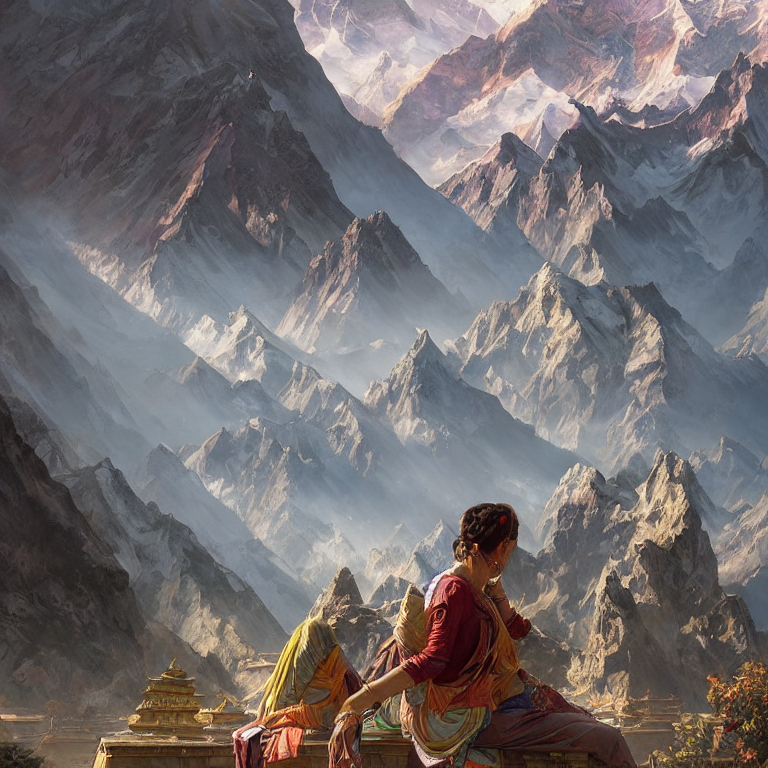
\includegraphics[width=0.3\linewidth]{static/sample_imgs/main_1x2/nepal_0.png} & 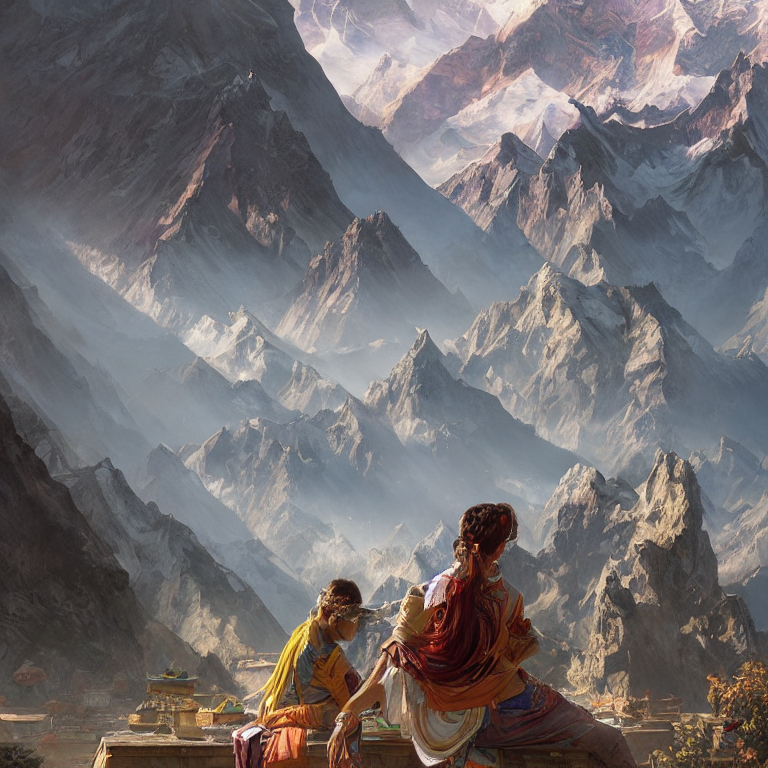
\includegraphics[width=0.3\linewidth]{static/sample_imgs/main_1x2/nepal_20.png} &
    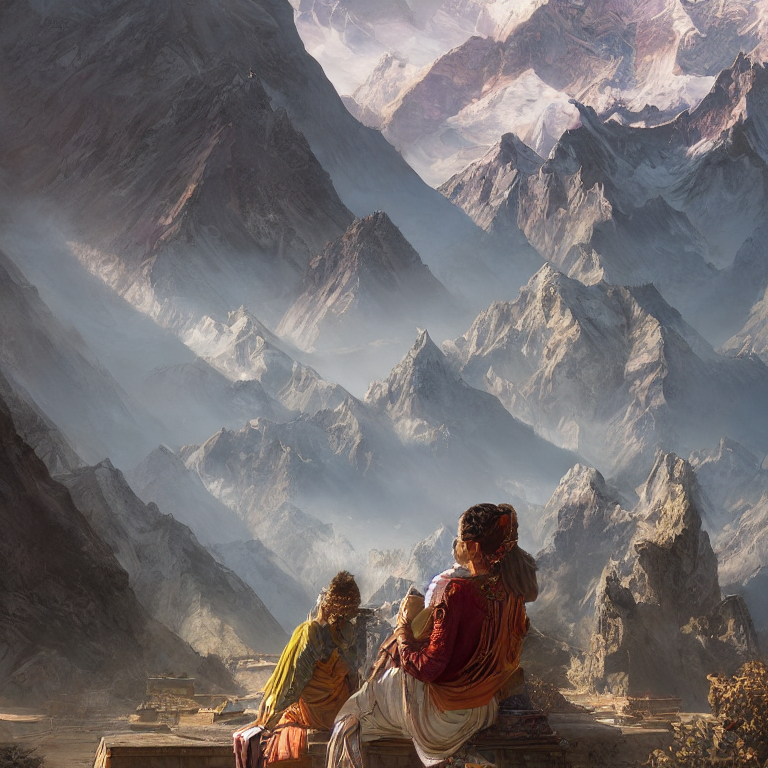
\includegraphics[width=0.3\linewidth]{static/sample_imgs/main_1x2/nepal_50.png}\\
    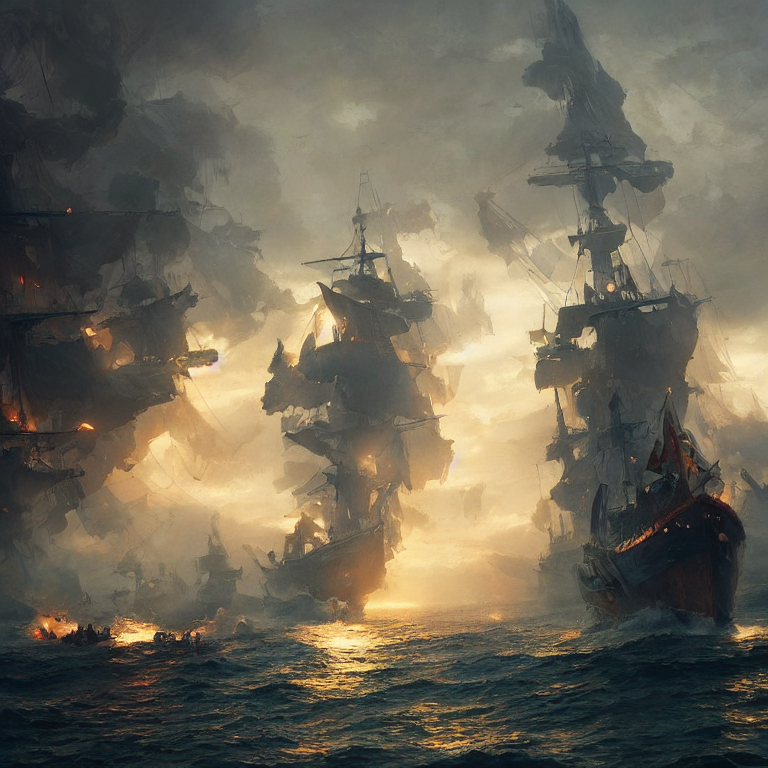
\includegraphics[width=0.3\linewidth]{static/sample_imgs/main_1x2/naval_0.png} & 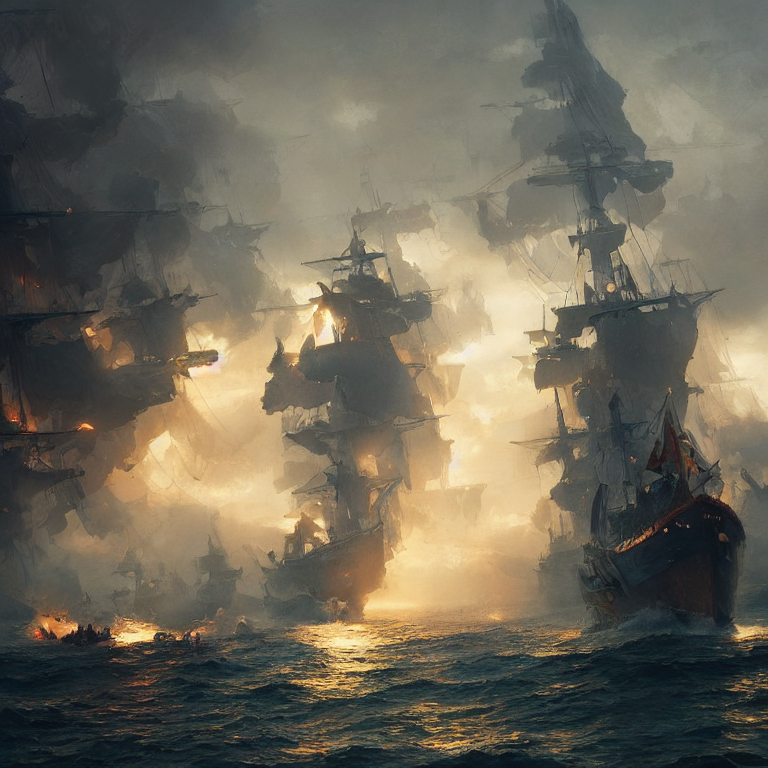
\includegraphics[width=0.3\linewidth]{static/sample_imgs/main_1x2/naval_20.png} &
    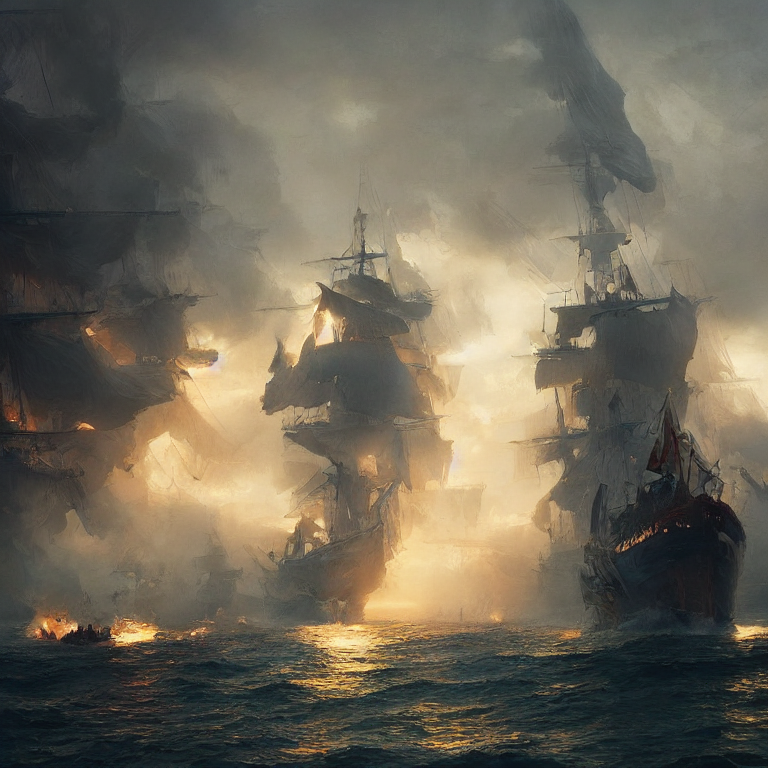
\includegraphics[width=0.3\linewidth]{static/sample_imgs/main_1x2/naval_50.png}\\
    \(r=0\%\) & \(50\%\) & \(50\%\) \\
\end{tabular}
\caption{$768 \times 768$ images created with the ToMe configured according to our best setup from \(3.2\)}
\end{table}

\newpage
\appendix
\pagenumbering{gobble}
\section{Data Tables}
\begin{table}
    \begin{minipage}{0.48\textwidth}
        \centering
        \begin{tabular}{|c|c|c|}
            \hline
            r\% & FID & FID \\
            \hline
            0 & 0 & 0 \\
            10 & 29.95 & 32.07 \\
            20 & 40.26 & 41.60 \\
            30 & 47.74 & 49.15 \\
            40 & 53.48 & 54.98 \\
            50 & 58.19 & 61.13 \\
            60 & 62.46 & 66.21 \\
            \hline
        \end{tabular}
        \caption{default vs all}
        \label{tab:table1}
    \end{minipage}
    \hfill
    \begin{minipage}{0.48\textwidth}
        \centering
        \begin{tabular}{|c|c|c|}
            \hline
            r\% & time (s/im) & time (s/im) \\
            \hline
            0 & 70.74 & 69.91 \\
            10 & 63.28 & 62.61 \\
            20 & 55.64 & 55.06 \\
            30 & 48.42 & 47.61 \\
            40 & 42.97 & 41.88 \\
            50 & 37.04 & 35.76 \\
            60 & 34.35 & 32.26 \\
            \hline
        \end{tabular}
        \caption{default vs all}
        \label{tab:table2}
    \end{minipage}
\end{table}

\begin{table}[htp]
\caption{default vs self-attn \& cross-attn vs self-attn \& mlp}
    \begin{minipage}{0.48\textwidth}
        \centering
        \begin{tabular}{|c||c|c|c|}
            \hline
            \multicolumn{1}{|c||}{r\%} & \multicolumn{3}{c|}{FID}\\
            \hline
            0 & 0 & 0 & 0 \\
            10 & 29.95 & 29.23 & 31.81 \\
            20 & 40.26 & 39.55 & 41.16 \\
            30 & 47.74 & 46.73 & 49.59 \\
            40 & 53.48 & 52.34 & 54.94 \\
            50 & 58.19 & 57.05 & 60.41 \\
            60 & 62.46 & 61.64 & 66.63 \\
            \hline
        \end{tabular}
    \end{minipage}
    \hfill
    \begin{minipage}{0.48\textwidth}
        \centering
        \begin{tabular}{|c||c|c|c|}
            \hline
            \multicolumn{1}{|c||}{r\%} & \multicolumn{3}{c|}{s/im}\\
            \hline
            0 & 70.74 & 69.75 & 73.88 \\
            10 & 63.28 & 62.46 & 65.41 \\
            20 & 55.64 & 54.98 & 57.20 \\
            30 & 48.42 & 47.92 & 49.41 \\
            40 & 42.97 & 42.02 & 42.83 \\
            50 & 37.04 & 36.23 & 36.51 \\
            60 & 34.35 & 32.93 & 33.08 \\
            \hline
        \end{tabular}
    \end{minipage}
\end{table}
\begin{table}[htp]
\caption{default vs cross-attn \& mlp vs only cross-attn}
    \begin{minipage}{0.48\textwidth}
        \centering
        \begin{tabular}{|c||c|c|c|}
            \hline
            \multicolumn{1}{|c||}{r\%} & \multicolumn{3}{c|}{FID}\\
            \hline
            0 & 0 & 0 & 0 \\
            10 & 29.95 & 21.46 & 3.05 \\
            20 & 40.26 & 32.45 & 4.29 \\
            30 & 47.74 & 39.86 & 6.01 \\
            40 & 53.48 & 46.06 & 7.49 \\
            50 & 58.19 & 52.48 & 9.50 \\
            60 & 62.46 & 57.71 & 11.16 \\
            \hline
        \end{tabular}
    \end{minipage}
    \hfill
    \begin{minipage}{0.48\textwidth}
        \centering
        \begin{tabular}{|c||c|c|c|}
            \hline
            \multicolumn{1}{|c||}{r\%} & \multicolumn{3}{c|}{s/im}\\
            \hline
            0 & 70.74 & 70.78 & 69.99 \\
            10 & 63.28 & 71.94 & 70.85 \\
            20 & 55.64 & 71.76 & 70.78 \\
            30 & 48.42 & 71.58 & 70.74 \\
            40 & 42.97 & 71.45 & 70.91 \\
            50 & 37.04 & 70.88 & 70.57 \\
            60 & 34.35 & 70.64 & 70.52 \\
            \hline
        \end{tabular}
    \end{minipage}
\end{table}
\begin{table}[htp]
\caption{default vs self-attn \& cross-attn (the second time)}
    \begin{minipage}{0.48\textwidth}
        \centering
        \begin{tabular}{|c||c|c|}
            \hline
            \multicolumn{1}{|c||}{r\%} & \multicolumn{2}{c|}{FID}\\
            \hline
            0 & 0 & 0 \\
            10 & 32.49 & 32.71 \\
            20 & 43.07 & 42.52 \\
            30 & 51.44 & 50.31 \\
            40 & 57.06 & 56.37 \\
            50 & 61.53 & 60.99 \\
            60 & 67.08 & 65.99 \\
            \hline
        \end{tabular}
    \end{minipage}
    \hfill
    \begin{minipage}{0.48\textwidth}
        \centering
        \begin{tabular}{|c||c|c|}
            \hline
            \multicolumn{1}{|c||}{r\%} & \multicolumn{2}{c|}{s/im}\\
            \hline
            0 & 70.77 & 70.02 \\
            10 & 63.44 & 62.67 \\
            20 & 55.85 & 55.39 \\
            30 & 48.63 & 48.01 \\
            40 & 43.22 & 42.11 \\
            50 & 37.53 & 36.56 \\
            60 & 34.29 & 33.38 \\
            \hline
        \end{tabular}
    \end{minipage}
\end{table}
\begin{table}[htp]
\caption{default vs self-attn \& cross-attn $(512 \times 512)$}
    \begin{minipage}{0.48\textwidth}
        \centering
        \begin{tabular}{|c||c|c|}
            \hline
            \multicolumn{1}{|c||}{r\%} & \multicolumn{2}{c|}{FID}\\
            \hline
            0 & 0 & 0 \\
            10 & 41.06 & 41.45 \\
            20 & 49.80 & 48.45 \\
            30 & 55.03 & 54.39 \\
            40 & 59.10 & 59.16 \\
            50 & 63.39 & 63.09 \\
            60 & 68.30 & 67.53 \\
            \hline
        \end{tabular}
    \end{minipage}
    \hfill
    \begin{minipage}{0.48\textwidth}
        \centering
        \begin{tabular}{|c||c|c|}
            \hline
            \multicolumn{1}{|c||}{r\%} & \multicolumn{2}{c|}{s/im}\\
            \hline
            0 & 16.92 & 17.61 \\
            10 & 18.08 & 18.39 \\
            20 & 16.31 & 16.70 \\
            30 & 15.32 & 15.59 \\
            40 & 14.35 & 14.67 \\
            50 & 12.93 & 13.33 \\
            60 & 12.75 & 12.86 \\
            \hline
        \end{tabular}
    \end{minipage}
\end{table}
\begin{table}[htp]
\caption{default ($2 \times 2$) vs $3 \times 3$ vs $1 \times 2$}
    \begin{minipage}{0.48\textwidth}
        \centering
        \begin{tabular}{|c||c|c|c|}
            \hline
            \multicolumn{1}{|c||}{r\%} & \multicolumn{3}{c|}{FID}\\
            \hline
            0 & 0 & 0 & 0 \\
            10 & 32.71 & 32.09 & 29.10 \\
            20 & 42.52 & 43.71 & 38.38 \\
            30 & 50.31 & 51.80 & 45.69 \\
            40 & 56.37 & 57.54 & 51.33 \\
            50 & 60.99 & 63.06 & 58.89 \\
            60 & 65.99 & 68.69 & - \\
            \hline
        \end{tabular}
    \end{minipage}
    \hfill
    \begin{minipage}{0.48\textwidth}
        \centering
        \begin{tabular}{|c||c|c|c|}
            \hline
            \multicolumn{1}{|c||}{r\%} & \multicolumn{3}{c|}{s/im}\\
            \hline
            0 & 70.02 & 69.56 & 69.34 \\
            10 & 62.67 & 61.92 & 62.39 \\
            20 & 55.39 & 54.44 & 54.94 \\
            30 & 48.01 & 47.09 & 47.59 \\
            40 & 42.11 & 41.43 & 42.24 \\
            50 & 36.56 & 35.62 & 36.27 \\
            60 & 33.38 & 32.37 & - \\
            \hline
        \end{tabular}
    \end{minipage}
\end{table}
\begin{table}[htp]
\caption{only self-attn with $2 \times 2$ vs self-attn \& cross-attn with $2 \times 2$ vs self-attn \& cross-attn with $1 \times 2$}
    \begin{minipage}{0.48\textwidth}
        \centering
        \begin{tabular}{|c||c|c|c|}
            \hline
            \multicolumn{1}{|c||}{r\%} & \multicolumn{3}{c|}{FID}\\
            \hline
            0 & 0 & 0 & 0 \\
            10 & 31.33 & 30.97 & 27.80 \\
            20 & 41.67 & 41.04 & 36.93 \\
            30 & 49.59 & 48.52 & 44.36 \\
            40 & 55.27 & 54.36 & 49.99 \\
            50 & 59.86 & 59.02 & 57.76 \\
            60 & 64.77 & 63.82 & - \\
            \hline
        \end{tabular}
    \end{minipage}
    \hfill
    \begin{minipage}{0.48\textwidth}
        \centering
        \begin{tabular}{|c||c|c|c|}
            \hline
            \multicolumn{1}{|c||}{r\%} & \multicolumn{3}{c|}{s/im}\\
            \hline
            0 & 70.76 & 69.88 & 71.25 \\
            10 & 63.36 & 62.57 & 64.05 \\
            20 & 55.75 & 55.19 & 55.88 \\
            30 & 48.53 & 47.97 & 48.49 \\
            40 & 43.10 & 42.07 & 43.38 \\
            50 & 37.29 & 36.40 & 36.75 \\
            60 & 34.32 & 33.16 & - \\
            \hline
        \end{tabular}
    \end{minipage}
\end{table}
\newpage

\newpage
\section{Images}
\begin{table}[!htb]
\centering
\begin{tabular}{c c@{}c@{}c@{}c@{}c@{}c}
    
\includegraphics[width=0.135\linewidth]{chapter/appendix/def_imgs/yorke/y_0.png} & 
    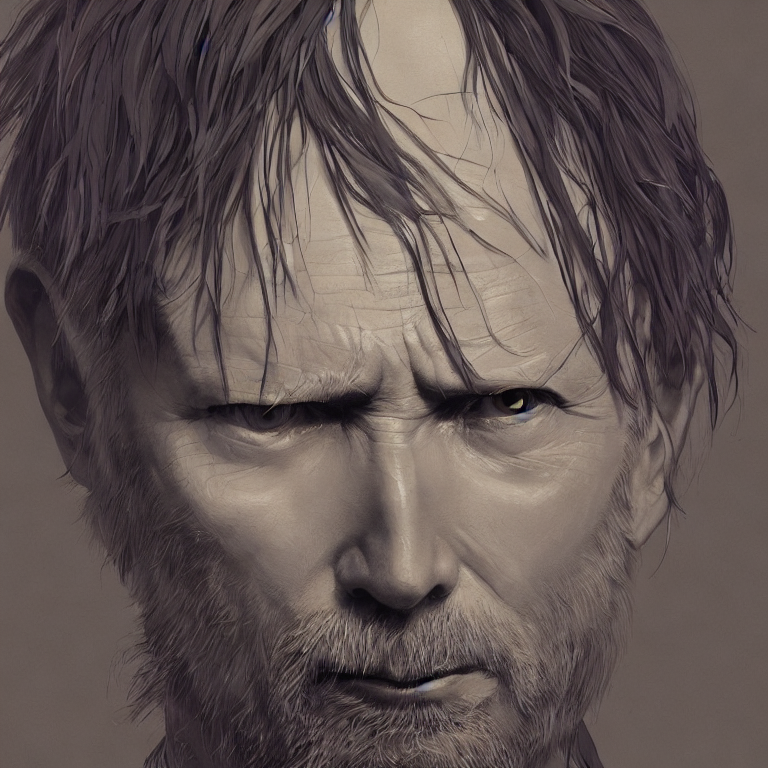
\includegraphics[width=0.135\linewidth]{chapter/appendix/def_imgs/yorke/y_10.png} &
    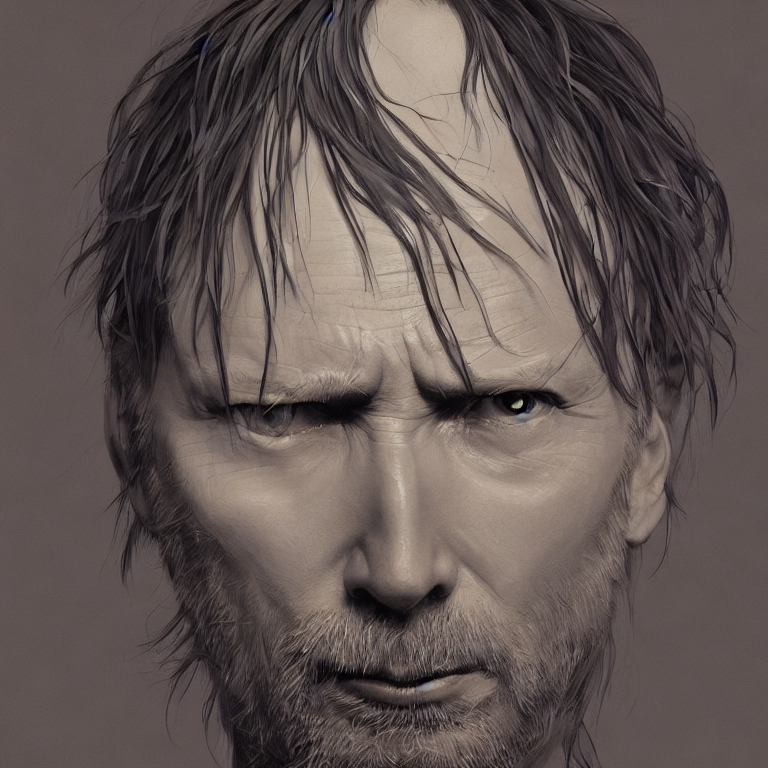
\includegraphics[width=0.135\linewidth]{chapter/appendix/def_imgs/yorke/y_20.png} &
    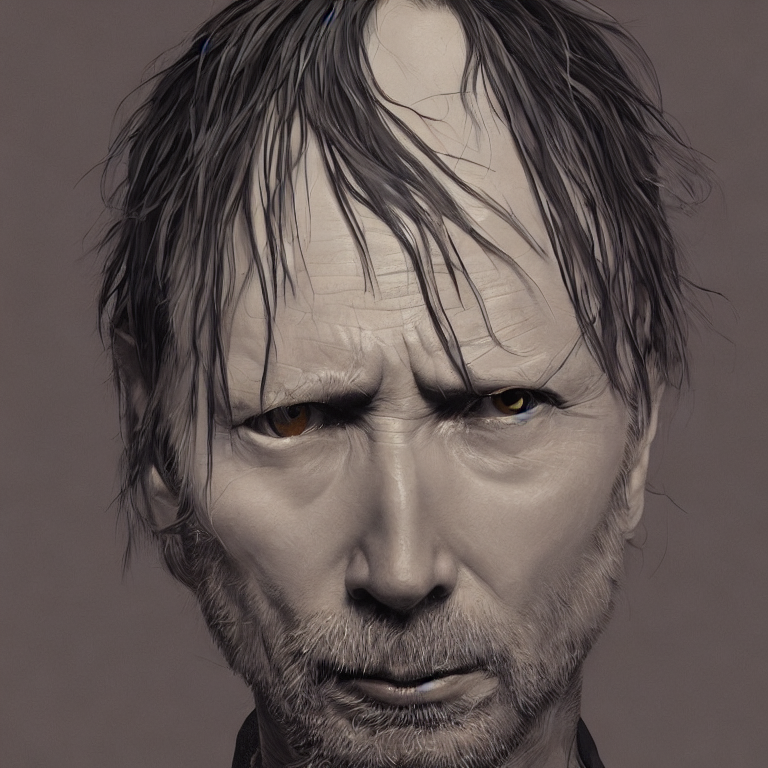
\includegraphics[width=0.135\linewidth]{chapter/appendix/def_imgs/yorke/y_30.png} &
    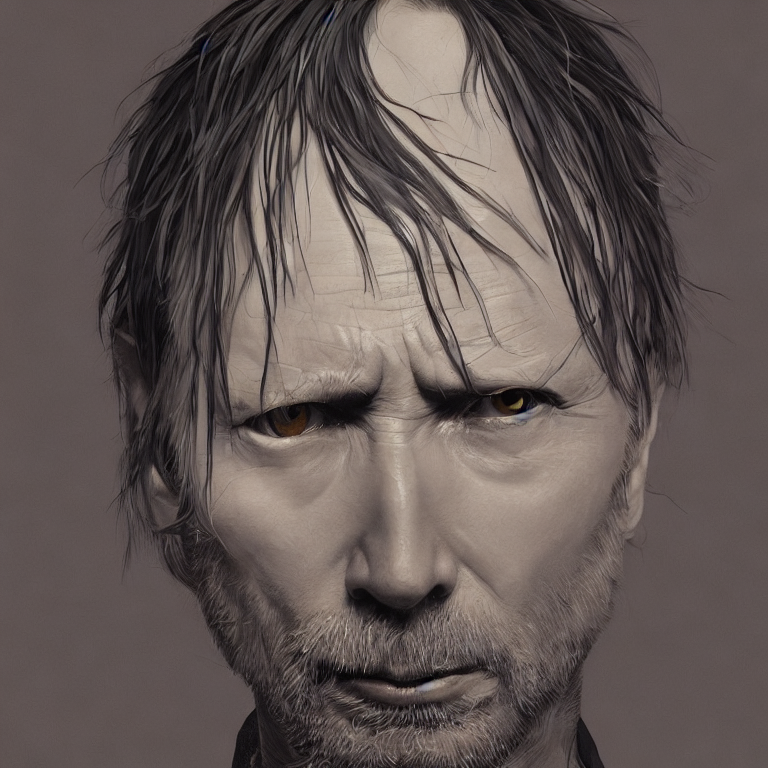
\includegraphics[width=0.135\linewidth]{chapter/appendix/def_imgs/yorke/y_40.png} &
    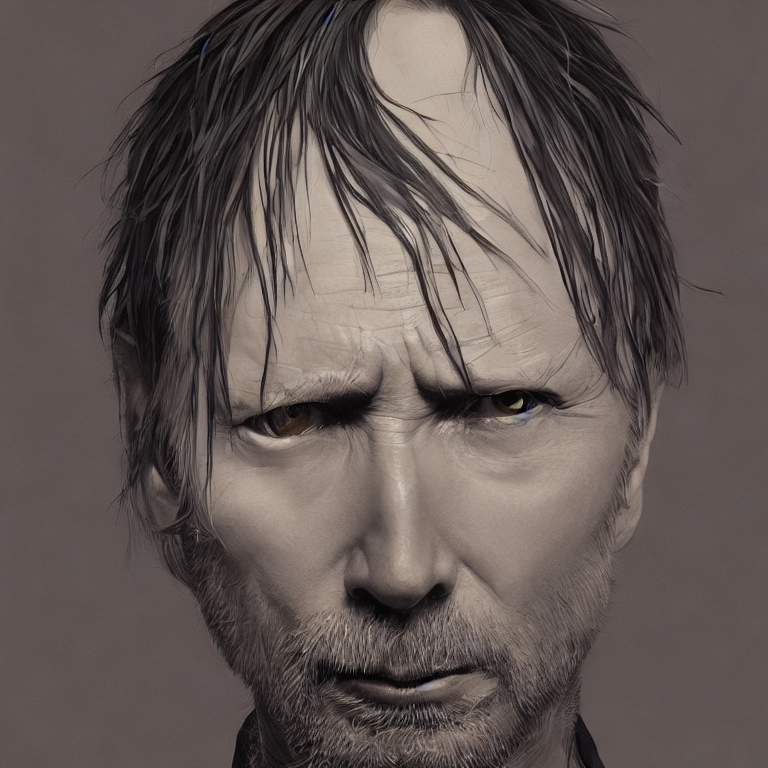
\includegraphics[width=0.135\linewidth]{chapter/appendix/def_imgs/yorke/y_50.png} &
    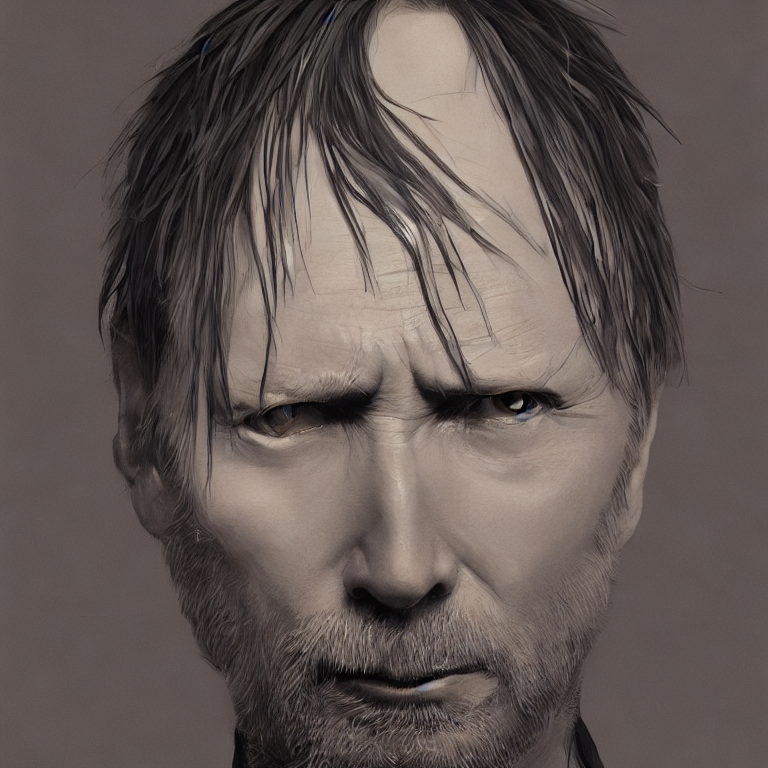
\includegraphics[width=0.135\linewidth]{chapter/appendix/def_imgs/yorke/y_60.png} \\
    
\includegraphics[width=0.135\linewidth]{chapter/appendix/def_imgs/woman/w_0.png} & 
    
\includegraphics[width=0.135\linewidth]{chapter/appendix/def_imgs/woman/w_10.png} &
    
\includegraphics[width=0.135\linewidth]{chapter/appendix/def_imgs/woman/w_20.png} &
    
\includegraphics[width=0.135\linewidth]{chapter/appendix/def_imgs/woman/w_30.png} &
    
\includegraphics[width=0.135\linewidth]{chapter/appendix/def_imgs/woman/w_40.png} &
    
\includegraphics[width=0.135\linewidth]{chapter/appendix/def_imgs/woman/w_50.png} &
    
\includegraphics[width=0.135\linewidth]{chapter/appendix/def_imgs/woman/w_60.png} \\
    
\includegraphics[width=0.135\linewidth]{chapter/appendix/def_imgs/fairy/f_0.png} & 
    
\includegraphics[width=0.135\linewidth]{chapter/appendix/def_imgs/fairy/f_10.png} &
    
\includegraphics[width=0.135\linewidth]{chapter/appendix/def_imgs/fairy/f_20.png} &
    
\includegraphics[width=0.135\linewidth]{chapter/appendix/def_imgs/fairy/f_30.png} &
    
\includegraphics[width=0.135\linewidth]{chapter/appendix/def_imgs/fairy/f_40.png} &
    
\includegraphics[width=0.135\linewidth]{chapter/appendix/def_imgs/fairy/f_50.png} &
    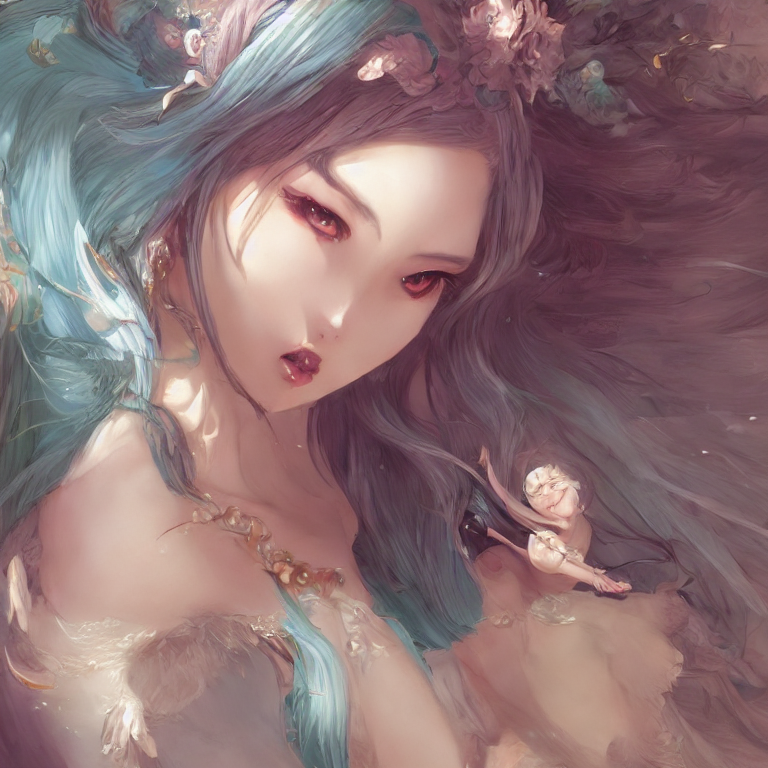
\includegraphics[width=0.135\linewidth]{chapter/appendix/def_imgs/fairy/f_60.png} \\
    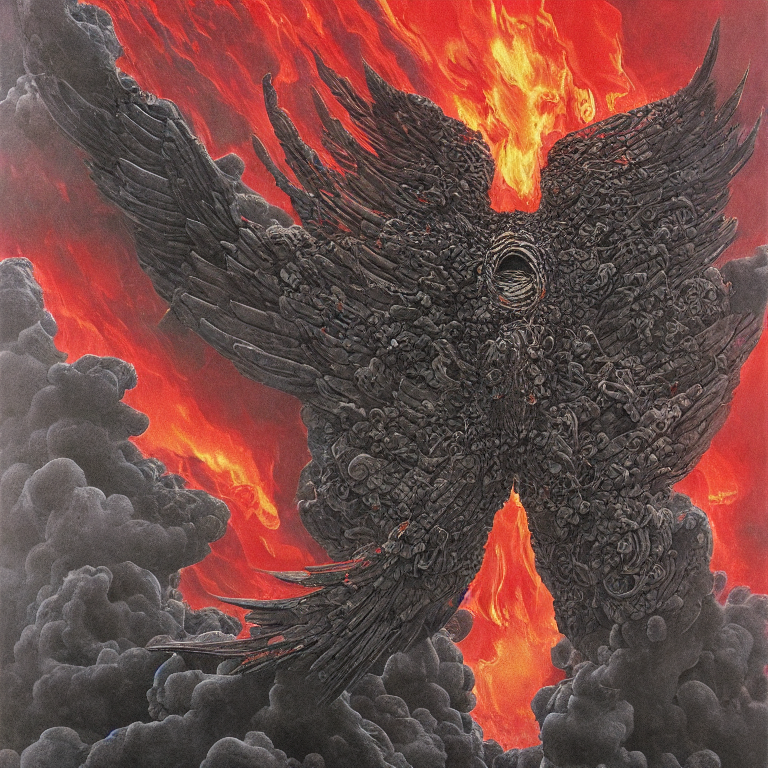
\includegraphics[width=0.135\linewidth]{chapter/appendix/def_imgs/phoenix/p_0.png} & 
    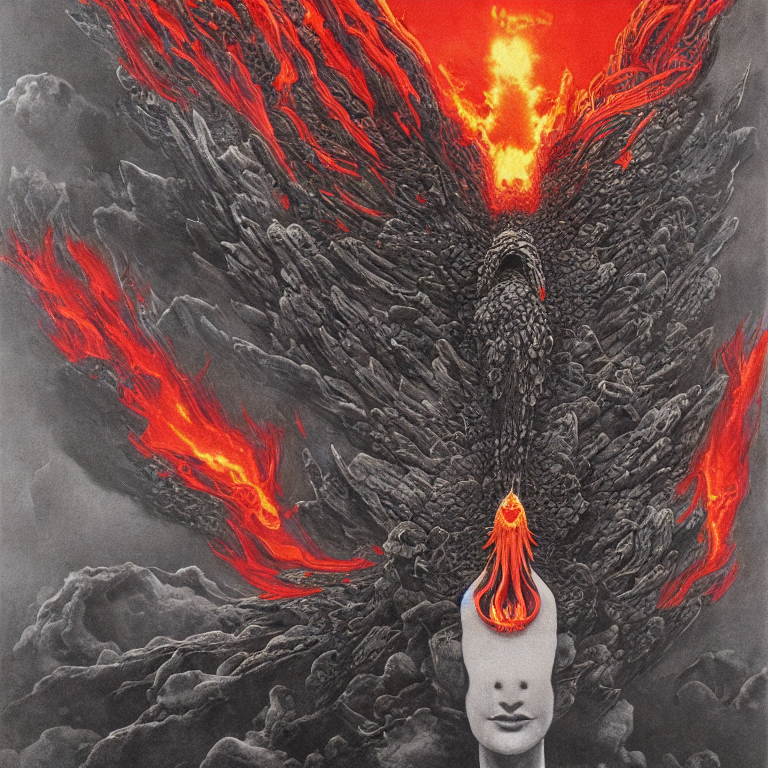
\includegraphics[width=0.135\linewidth]{chapter/appendix/def_imgs/phoenix/p_10.png} &
    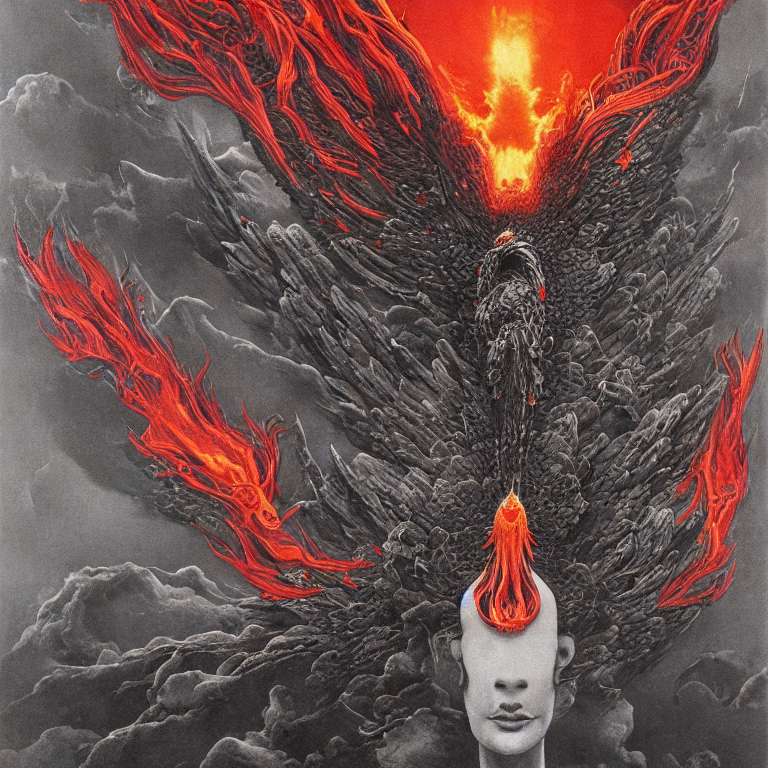
\includegraphics[width=0.135\linewidth]{chapter/appendix/def_imgs/phoenix/p_20.png} &
    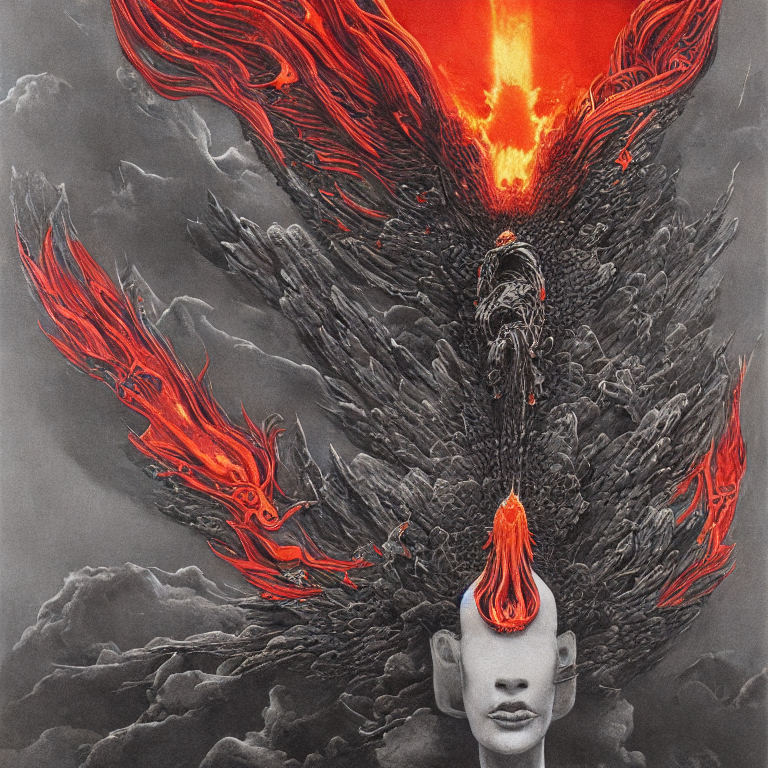
\includegraphics[width=0.135\linewidth]{chapter/appendix/def_imgs/phoenix/p_30.png} &
    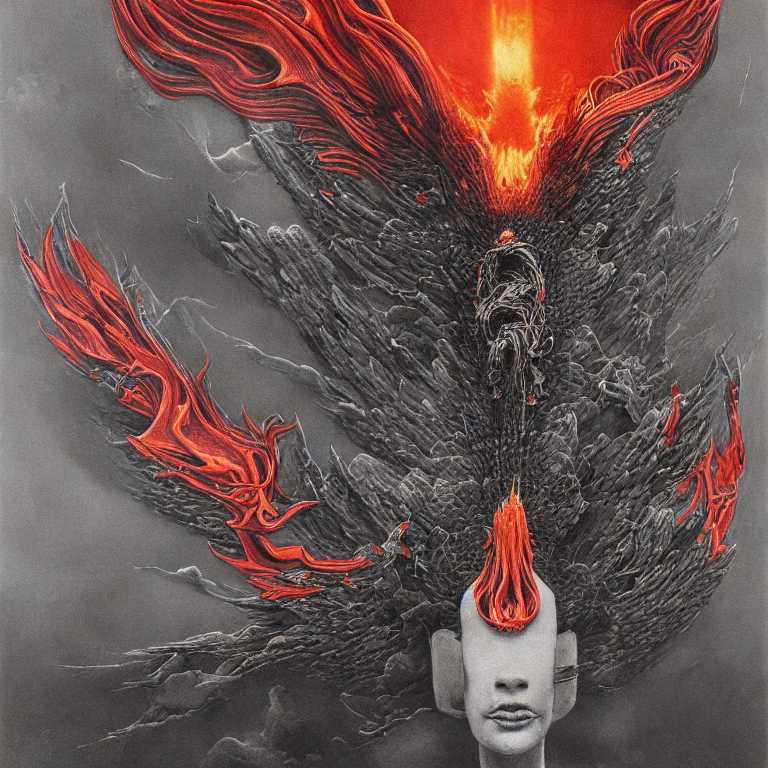
\includegraphics[width=0.135\linewidth]{chapter/appendix/def_imgs/phoenix/p_40.png} &
    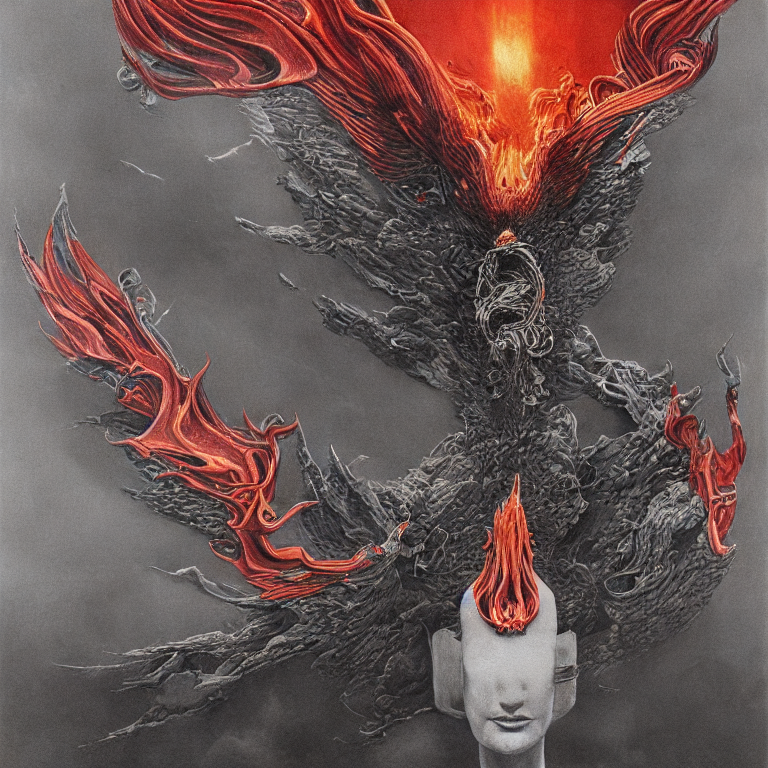
\includegraphics[width=0.135\linewidth]{chapter/appendix/def_imgs/phoenix/p_50.png} &
    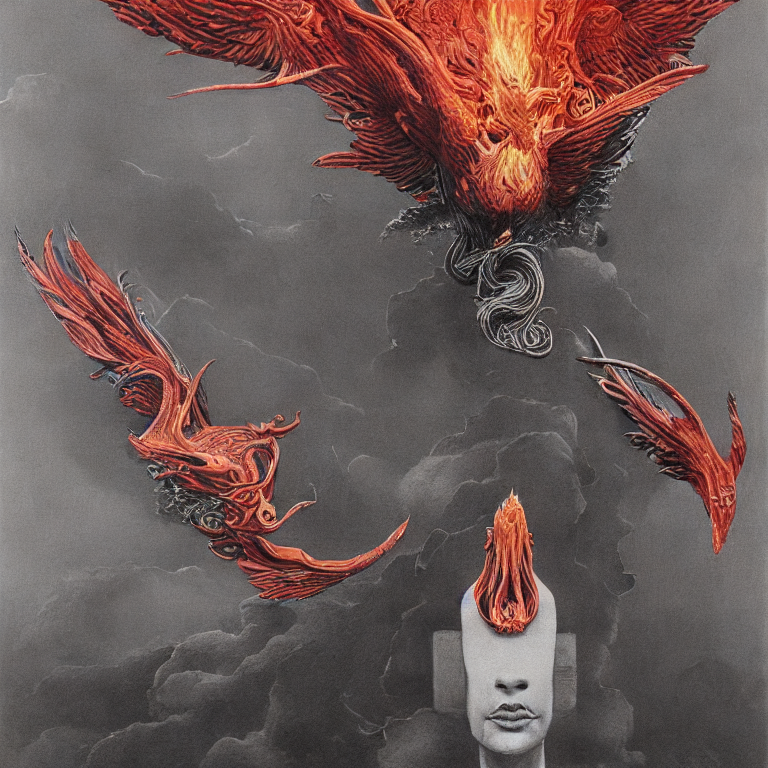
\includegraphics[width=0.135\linewidth]{chapter/appendix/def_imgs/phoenix/p_60.png} \\
    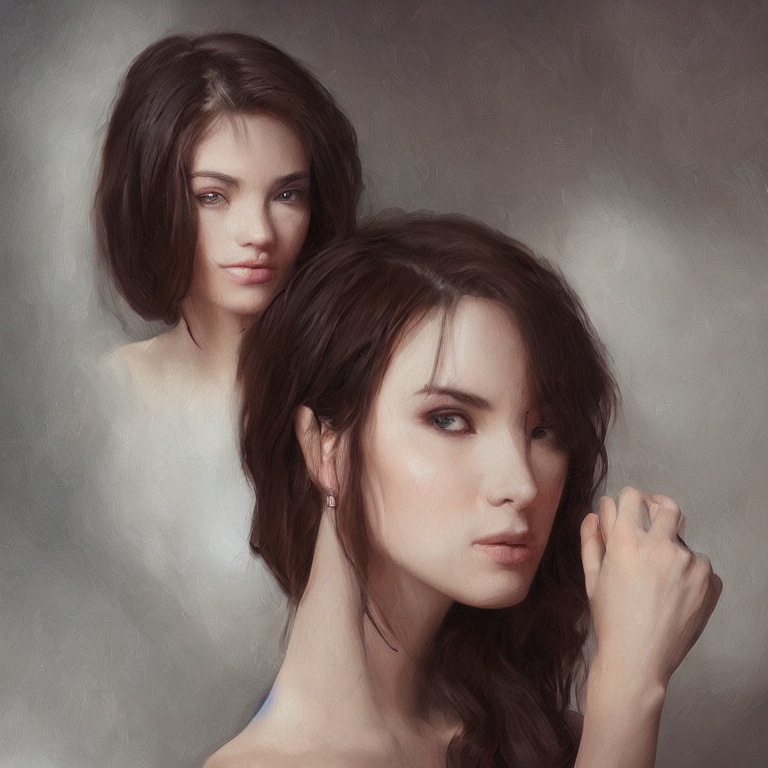
\includegraphics[width=0.135\linewidth]{chapter/appendix/def_imgs/woman2/w2_0.png} & 
    
\includegraphics[width=0.135\linewidth]{chapter/appendix/def_imgs/woman2/w2_10.png} &
    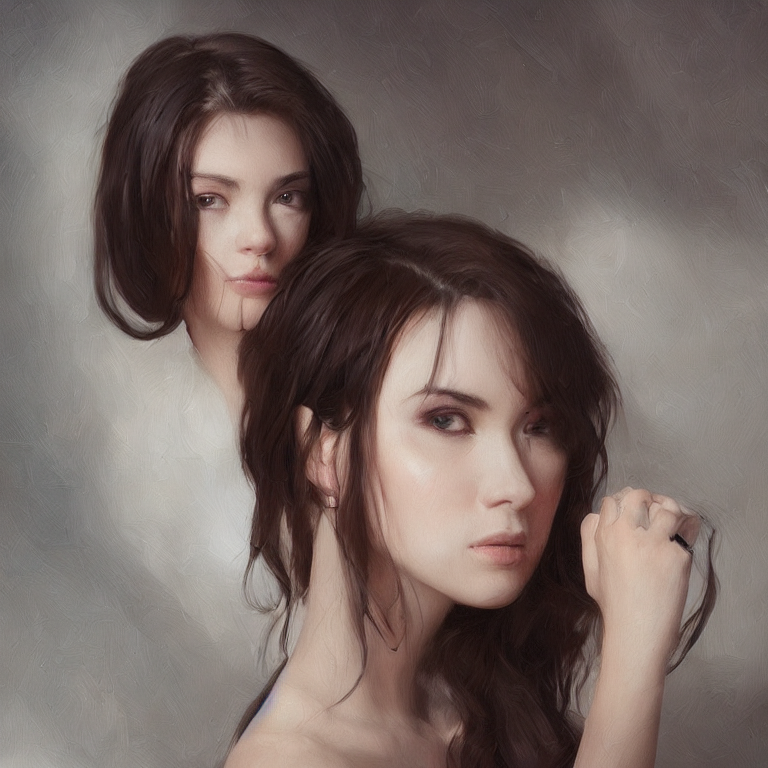
\includegraphics[width=0.135\linewidth]{chapter/appendix/def_imgs/woman2/w2_20.png} &
    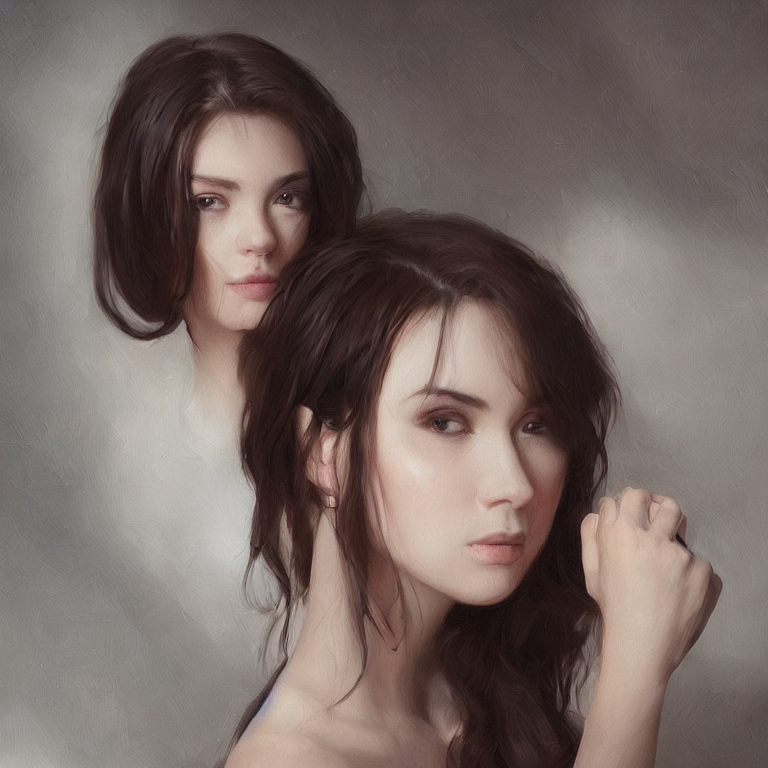
\includegraphics[width=0.135\linewidth]{chapter/appendix/def_imgs/woman2/w2_30.png} &
    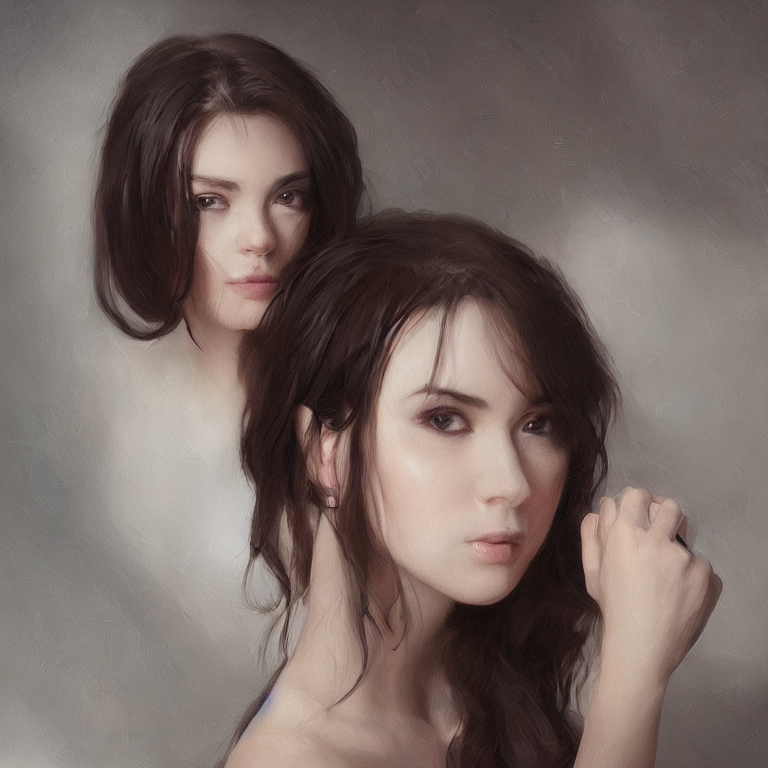
\includegraphics[width=0.135\linewidth]{chapter/appendix/def_imgs/woman2/w2_40.png} &
    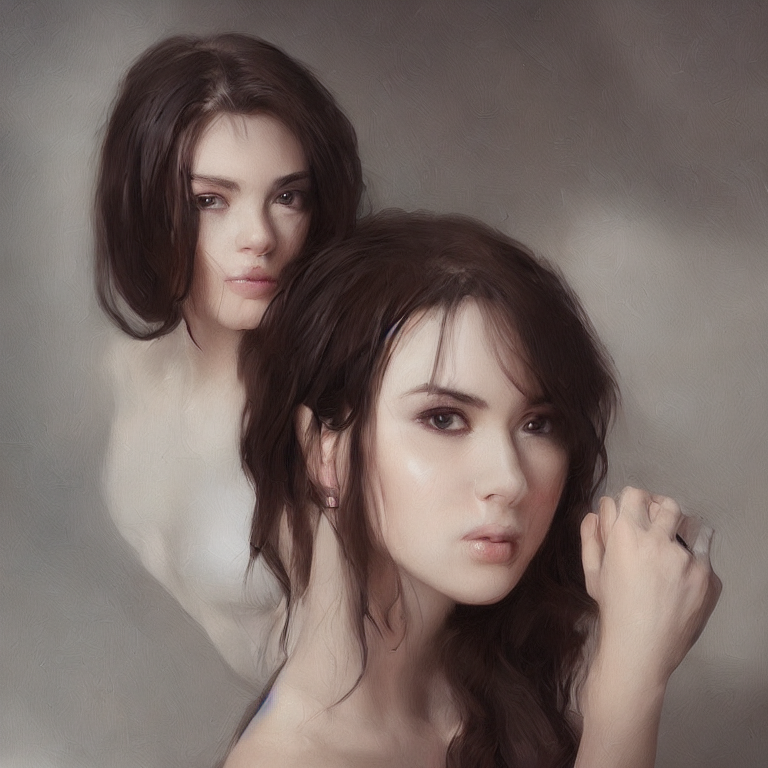
\includegraphics[width=0.135\linewidth]{chapter/appendix/def_imgs/woman2/w2_50.png} &
    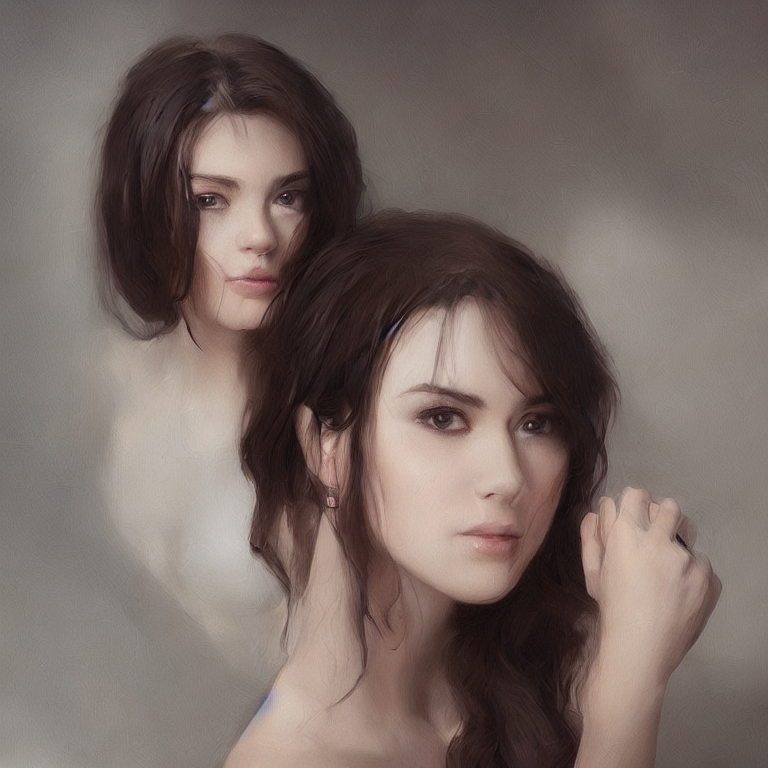
\includegraphics[width=0.135\linewidth]{chapter/appendix/def_imgs/woman2/w2_60.png} \\
    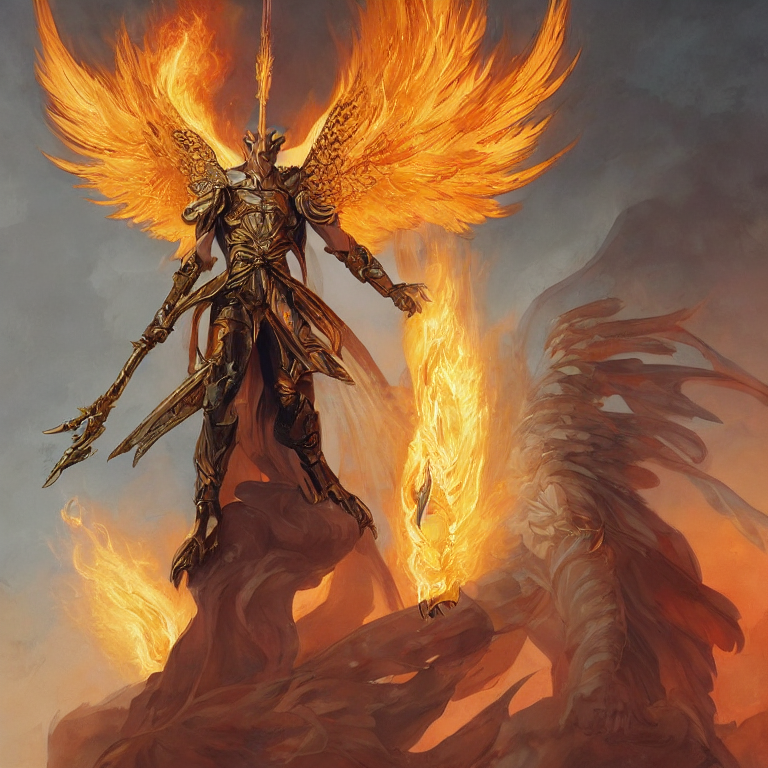
\includegraphics[width=0.135\linewidth]{chapter/appendix/def_imgs/angel/a_0.png} & 
    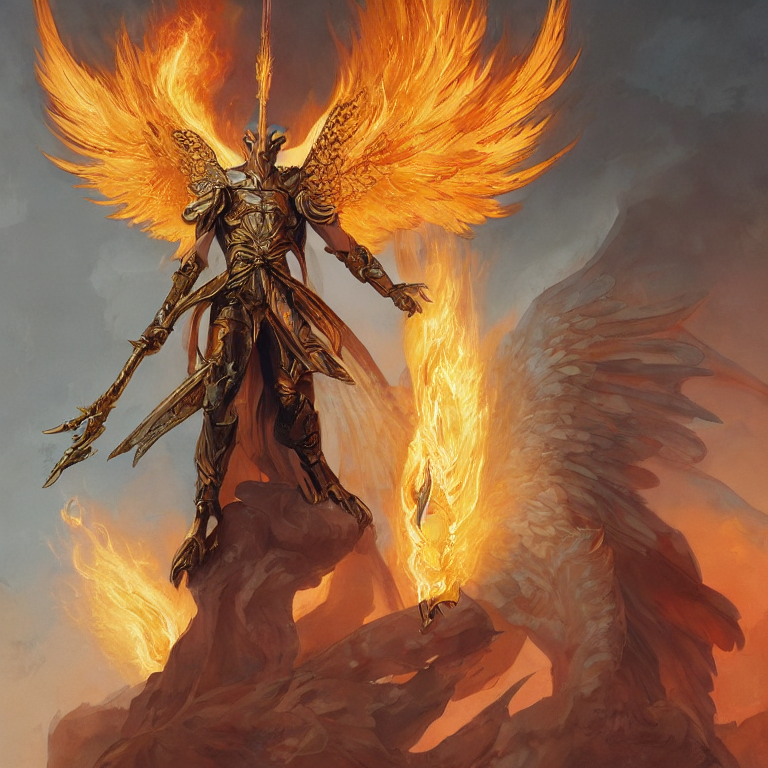
\includegraphics[width=0.135\linewidth]{chapter/appendix/def_imgs/angel/a_10.png} &
    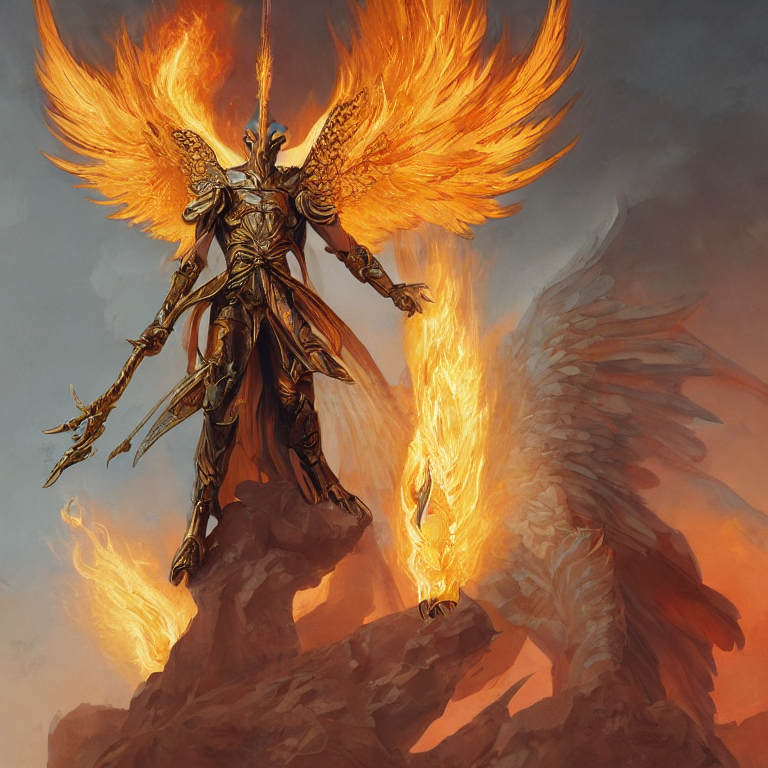
\includegraphics[width=0.135\linewidth]{chapter/appendix/def_imgs/angel/a_20.png} &
    \includegraphics[width=0.135\linewidth]{chapter/appendix/def_imgs/angel/a_30.png} &
    \includegraphics[width=0.135\linewidth]{chapter/appendix/def_imgs/angel/a_40.png} &
    \includegraphics[width=0.135\linewidth]{chapter/appendix/def_imgs/angel/a_50.png} &
    \includegraphics[width=0.135\linewidth]{chapter/appendix/def_imgs/angel/a_60.png} \\
    \includegraphics[width=0.135\linewidth]{chapter/appendix/def_imgs/cyberpunk/c_0.png} &
    \includegraphics[width=0.135\linewidth]{chapter/appendix/def_imgs/cyberpunk/c_10.png} &
    \includegraphics[width=0.135\linewidth]{chapter/appendix/def_imgs/cyberpunk/c_20.png} &
    \includegraphics[width=0.135\linewidth]{chapter/appendix/def_imgs/cyberpunk/c_30.png} &
    \includegraphics[width=0.135\linewidth]{chapter/appendix/def_imgs/cyberpunk/c_40.png} &
    \includegraphics[width=0.135\linewidth]{chapter/appendix/def_imgs/cyberpunk/c_50.png} &
    \includegraphics[width=0.135\linewidth]{chapter/appendix/def_imgs/cyberpunk/c_60.png} \\
    \includegraphics[width=0.135\linewidth]{chapter/appendix/def_imgs/tiefling/t_0.png} &
    \includegraphics[width=0.135\linewidth]{chapter/appendix/def_imgs/tiefling/t_10.png} &
    \includegraphics[width=0.135\linewidth]{chapter/appendix/def_imgs/tiefling/t_20.png} &
    \includegraphics[width=0.135\linewidth]{chapter/appendix/def_imgs/tiefling/t_30.png} &
    \includegraphics[width=0.135\linewidth]{chapter/appendix/def_imgs/tiefling/t_40.png} &
    \includegraphics[width=0.135\linewidth]{chapter/appendix/def_imgs/tiefling/t_50.png} &
    \includegraphics[width=0.135\linewidth]{chapter/appendix/def_imgs/tiefling/t_60.png} \\
    \(r=0\%\) & \(10\%\) & \(20\%\) & \(30\%\) & \(40\%\) & \(50\%\) & \(60\%\) \\
\end{tabular}
\caption{$768 \times 768$ images created with ToMe configuration according to our best setup from \(3.2\)}
\end{table}

\newpage
\section{Libraries and Code}
PyTorch: 1.13.0\\
Diffusers: 0.18.2\\
Transformers: 4.30.2\\
NumPy: 1.19.5\\
SciPy: 1.10.1\\
tomesd: 0.1.3\\
pytorch-fid (fork): 0.3.0\\
\\
Code for image generation (file: src/gen\_imgs.py):
\begin{lstlisting}[language=Python]
import sys       
sys.path.insert(1, '/gpfs/project/hebal100/ba-code')
from diffusers import DiffusionPipeline
import torch, time, random, string, tomesd, numpy as np, pandas as pd

HPC_PATH = "/gpfs/scratch/hebal100"

# save command line args
assert len(sys.argv) >= 5
MAIN_DIR = sys.argv[1]                      
sample_size = int(sys.argv[2])            
x, y =  int(sys.argv[3]), int(sys.argv[4]) 
try:
    src_file = sys.argv[5]                
except IndexError:
    src_file = None          

# load prompts and generate seeds
if src_file == None:
    all_prompts = pd.read_csv('data/prompts.csv')['colummn'].values
    idcs = np.random.randint(0, len(all_prompts), sample_size)
    prompts = all_prompts[idcs]
    seeds = np.random.randint(0, 4294967295, len(prompts))
# load prompts and seeds from previous run
else:
    prompts = pd.read_csv(f'{HPC_PATH}/data/{src_file}')['prompt'].values
    seeds = pd.read_csv(f'{HPC_PATH}/data/{src_file}')['seed'].values

# method for cutting oversized prompts
def cut_prompt(prompt, max_len=300, delimiter=','):
    if len(prompt) <= max_len:
        return prompt
    
    idx = prompt[:max_len].rfind(delimiter)
    # catch if delimiter isn't used
    if idx <= 0:
        idx = prompt[:max_len].rfind(' ')

    return prompt[:idx]

# build pipeline
assert torch.cuda.is_available()
pipeline = DiffusionPipeline.from_pretrained('pipelines/SD-v1-5').to('cuda')
pipeline.enable_attention_slicing()
# disable safety checker
def dummy(images, **kwargs):
    return images, [False]
pipeline.safety_checker = dummy

# set up lists
merge_volumes = [0, 0.1, 0.2, 0.3, 0.4, 0.5, 0.6]
directories = ['images_0', 'images_10', 'images_20', 'images_30', 'images_40', 'images_50', 'images_60']
logger = []

# run image generation loop to create image sets
for r, dir in zip(merge_volumes, directories):
    tomesd.apply_patch(pipeline, r, sx=2, sy=2, merge_attn=True, merge_crossattn=False, merge_mlp=False)
    for i in range(sample_size):
        prompt, seed = cut_prompt(prompts[i]), seeds[i].item()
        # create image
        start = time.time()
        image = pipeline(prompt, x, y, generator=torch.Generator().manual_seed(seed), ).images[0]
        end = time.time()
        diff_time = end - start
        # save image
        name = 'img_' + ''.join(random.choices(string.ascii_letters + string.digits, k=10))
        image.save(f'{HPC_PATH}/{MAIN_DIR}/{dir}/{name}.png')
        # create new log entry
        logger.append([prompt, seed, r, diff_time, name])       
tomesd.remove_patch(pipeline)

# save log
log = pd.DataFrame(logger, columns=['prompt', 'seed', 'm_vol', 'time', 'name'])
name = 'log_' + ''.join(random.choices(string.ascii_letters + string.digits, k=5))
log.to_csv(f'{HPC_PATH}/{MAIN_DIR}/logger/{name}.csv', index=False)
\end{lstlisting}
\vfill
Code for calculation of FID and average time (file: src/logging/gen\_perf\_log.py):
\begin{lstlisting}[language=Python]
import sys       
sys.path.insert(1, '/gpfs/project/hebal100/ba-code')
import pandas as pd
from libs.pytorch_fid.src.fid.fid_score import calculate_fid_given_paths

HPC_PATH = "/gpfs/scratch/hebal100"
DATA_PATH = sys.argv[1] 
# directories where images of certain merge volume are saved
directories = ['images_0', 'images_10', 'images_20', 'images_30', 'images_40', 'images_50', 'images_60']
m_vols = [0, 0.1, 0.2, 0.3, 0.4, 0.5, 0.6]
perf_values = []

for m_vol, dir in zip(m_vols, directories):
    fid = calculate_fid_given_paths((f'{HPC_PATH}/{DATA_PATH}/images_0', 
                                     f'{HPC_PATH}/{DATA_PATH}/{dir}'), batch_size=50, device='cuda', dims=2048)
    df = pd.read_csv(f'{HPC_PATH}/{DATA_PATH}/img_log.csv')
    df = df[df.m_vol == m_vol]
    avg_time = df['time'].values.mean()
    perf_values.append([m_vol, fid, avg_time])

perf_log = pd.DataFrame(perf_values, columns=['m_vol', 'fid', 'time'])
perf_log.to_csv(f'{HPC_PATH}/{DATA_PATH}/performance_log.csv', index=False)
\end{lstlisting}
\vfill

\newpage
\let\Section\section 
\def\section*#1{\Section{#1}} 
\bibliographystyle{apalike}
\bibliography{refs}


\end{document}